
\chapter{Per-Category Mass Plots}
\label{appendix:mass_plots}
\begin{figure}[h!]
    \begin{center}
        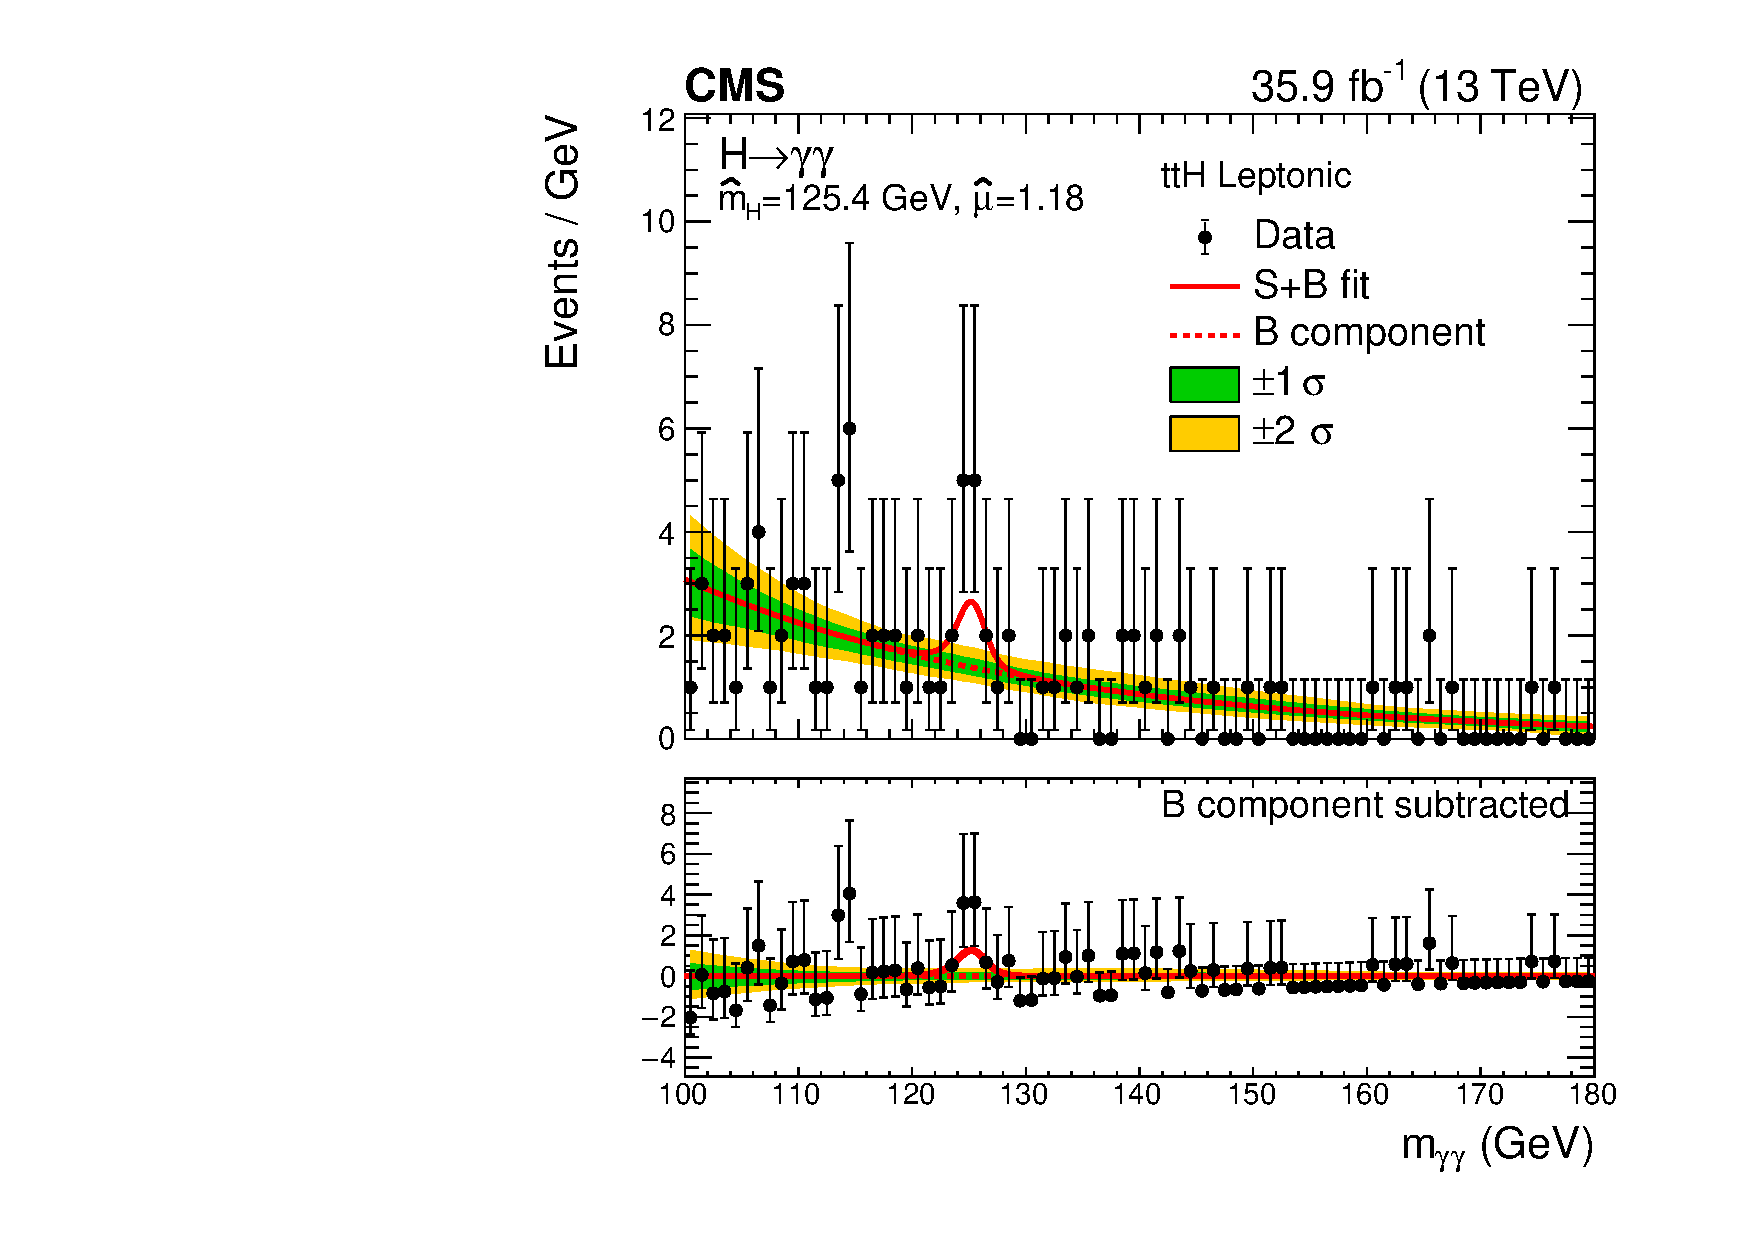
\includegraphics[width=0.47\textwidth]{figures/appendix_mass_plots/CMS-HIG-16-040_Figure_012-d.pdf}
        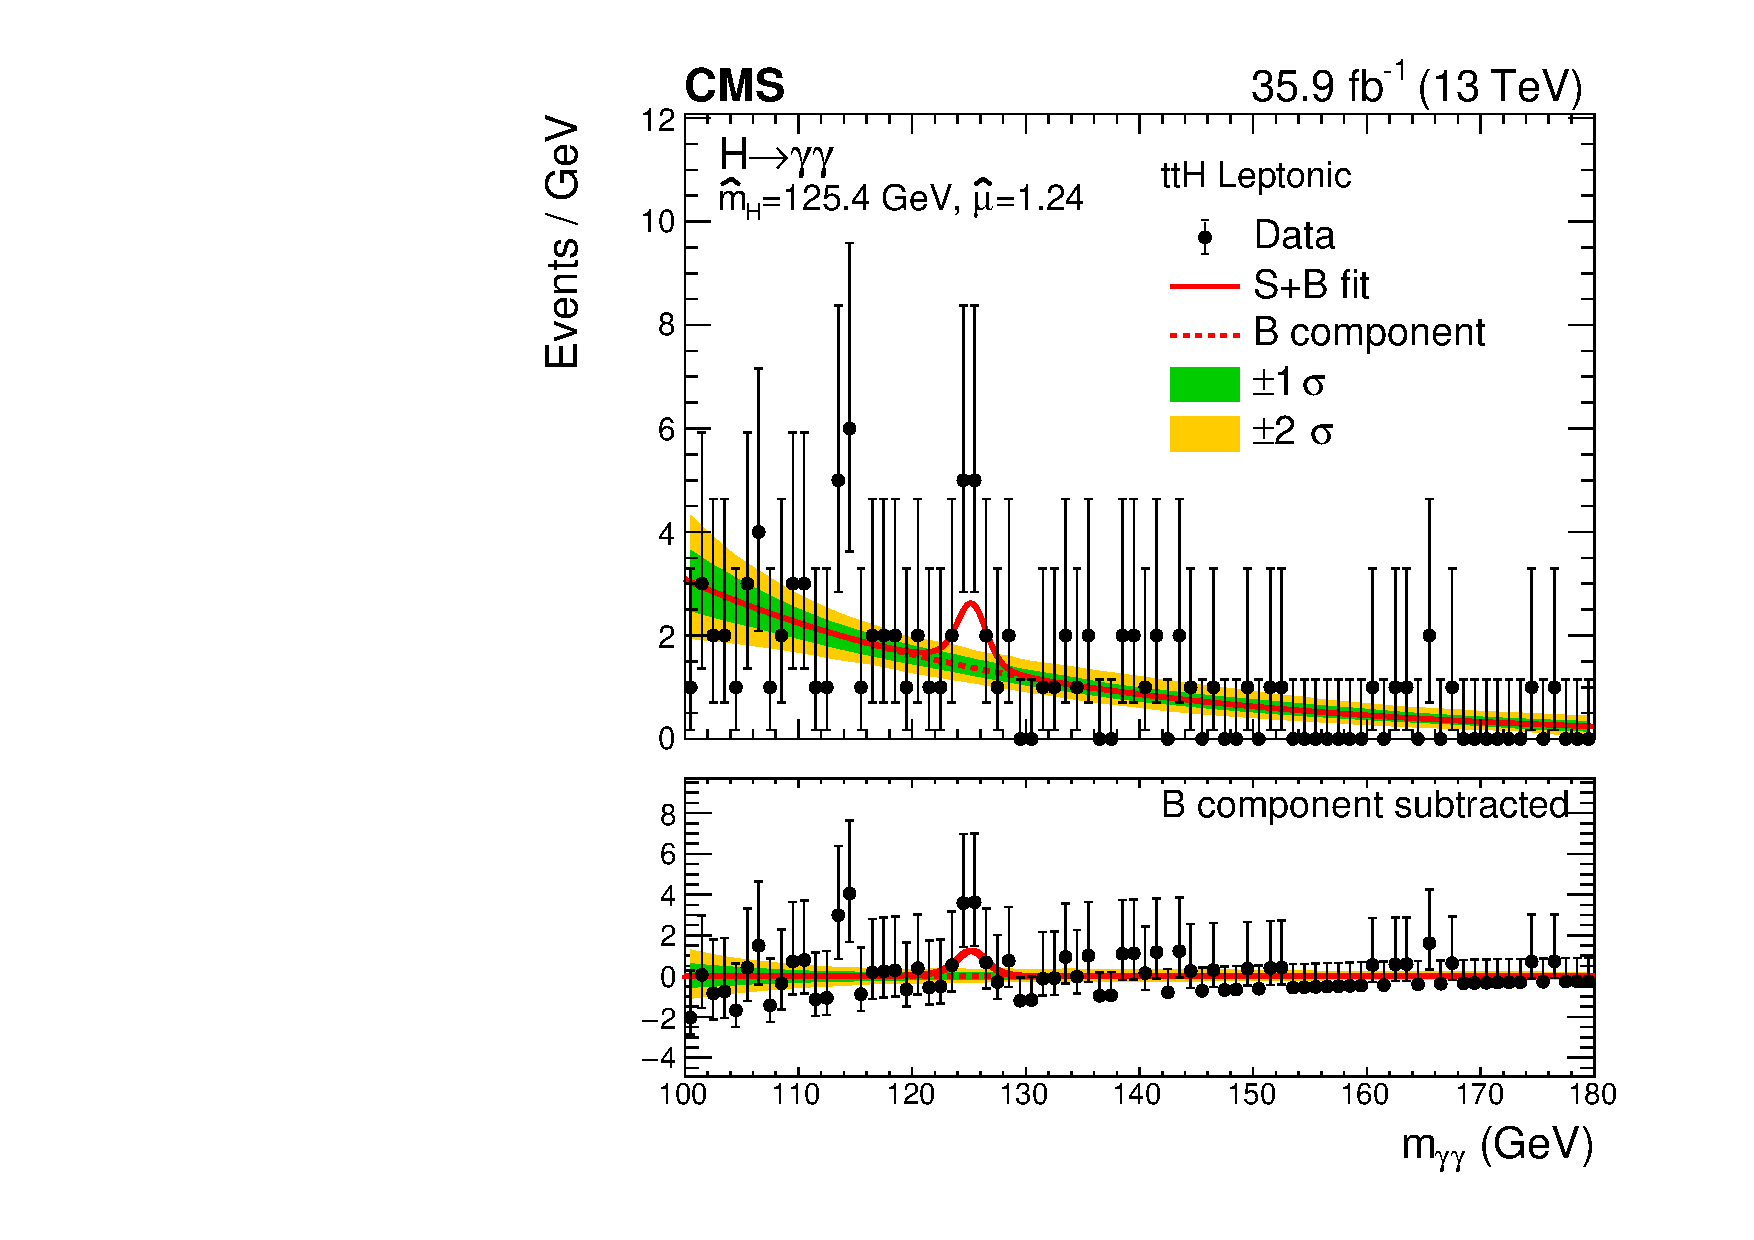
\includegraphics[width=0.47\textwidth]{figures/appendix_mass_plots/SBplots_jackWSnewOldTTHTTHLeptonicTag_13TeV.pdf}
    \end{center}
    \begin{center}
        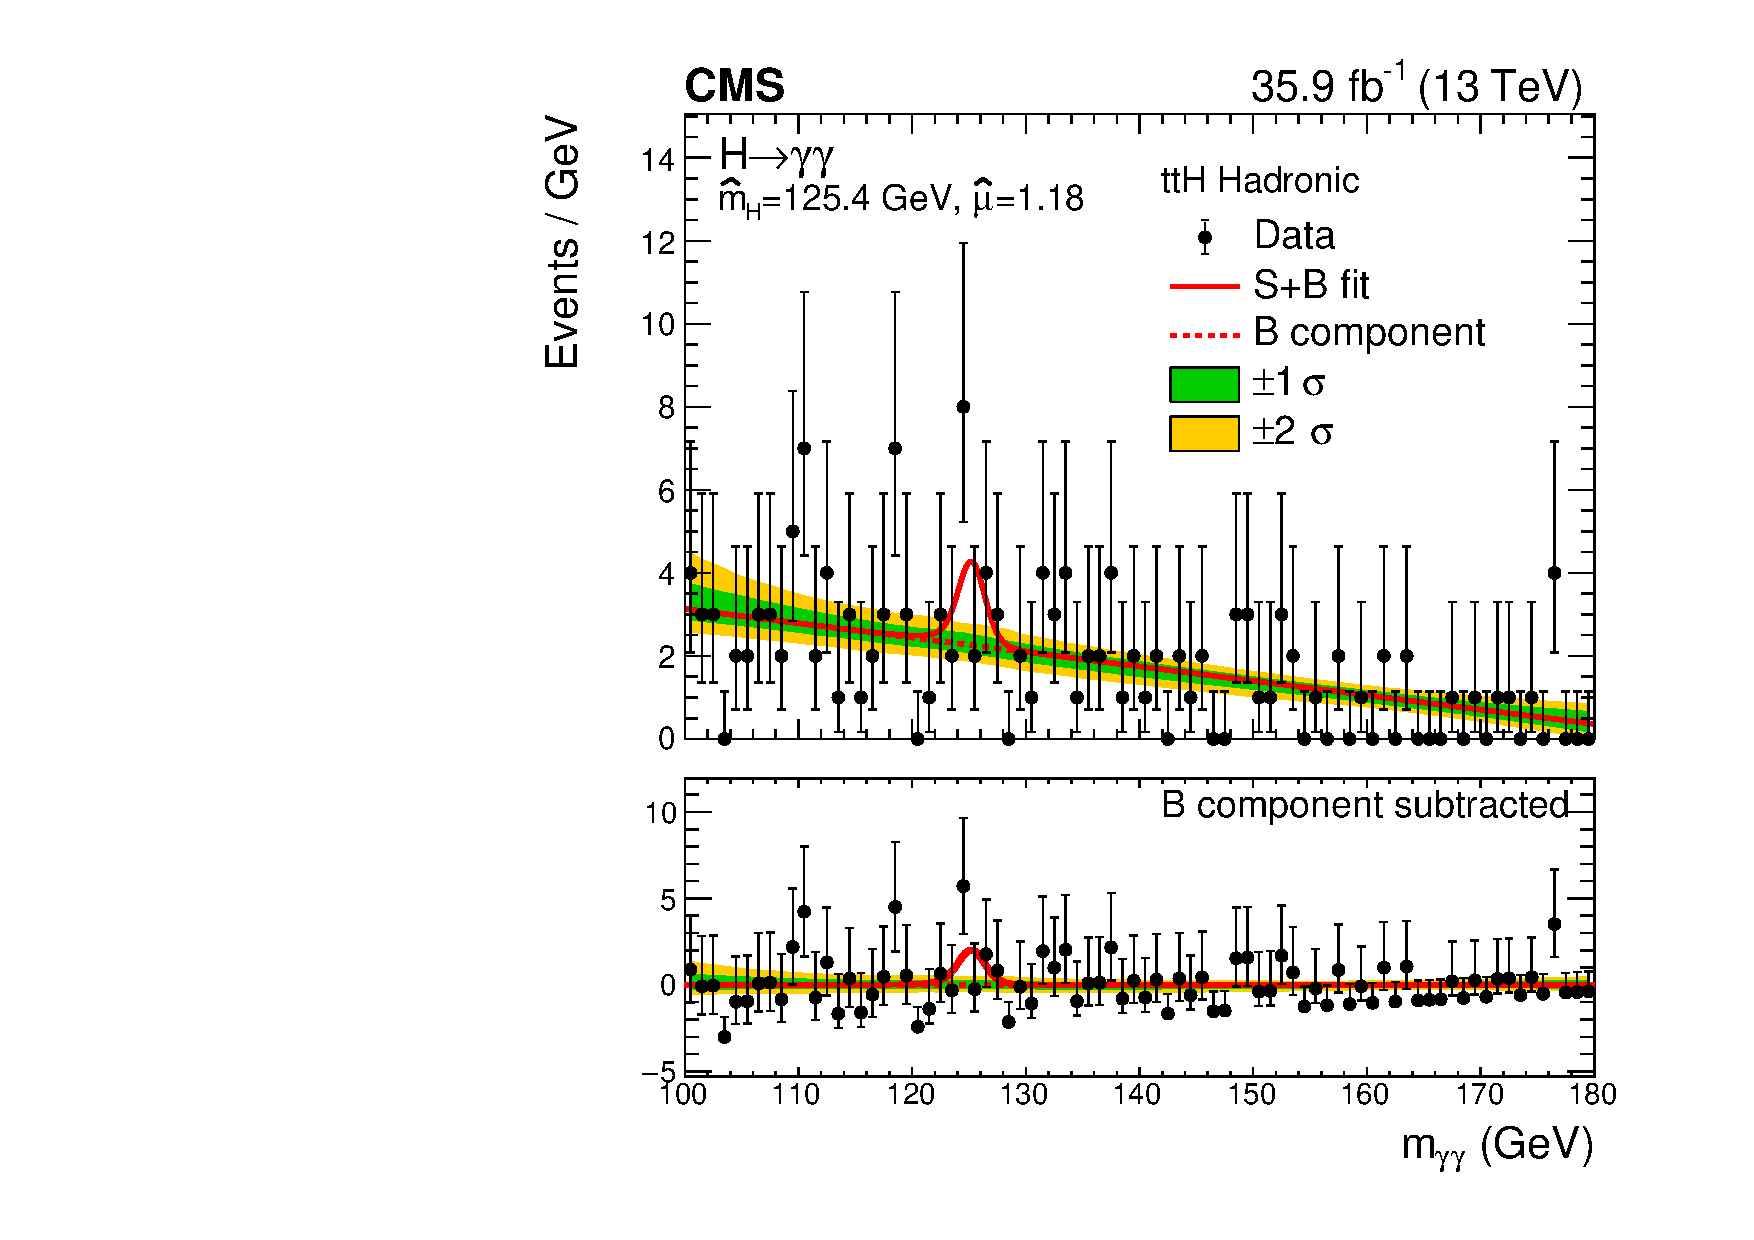
\includegraphics[width=0.47\textwidth]{figures/appendix_mass_plots/CMS-HIG-16-040_Figure_012-e.pdf}
        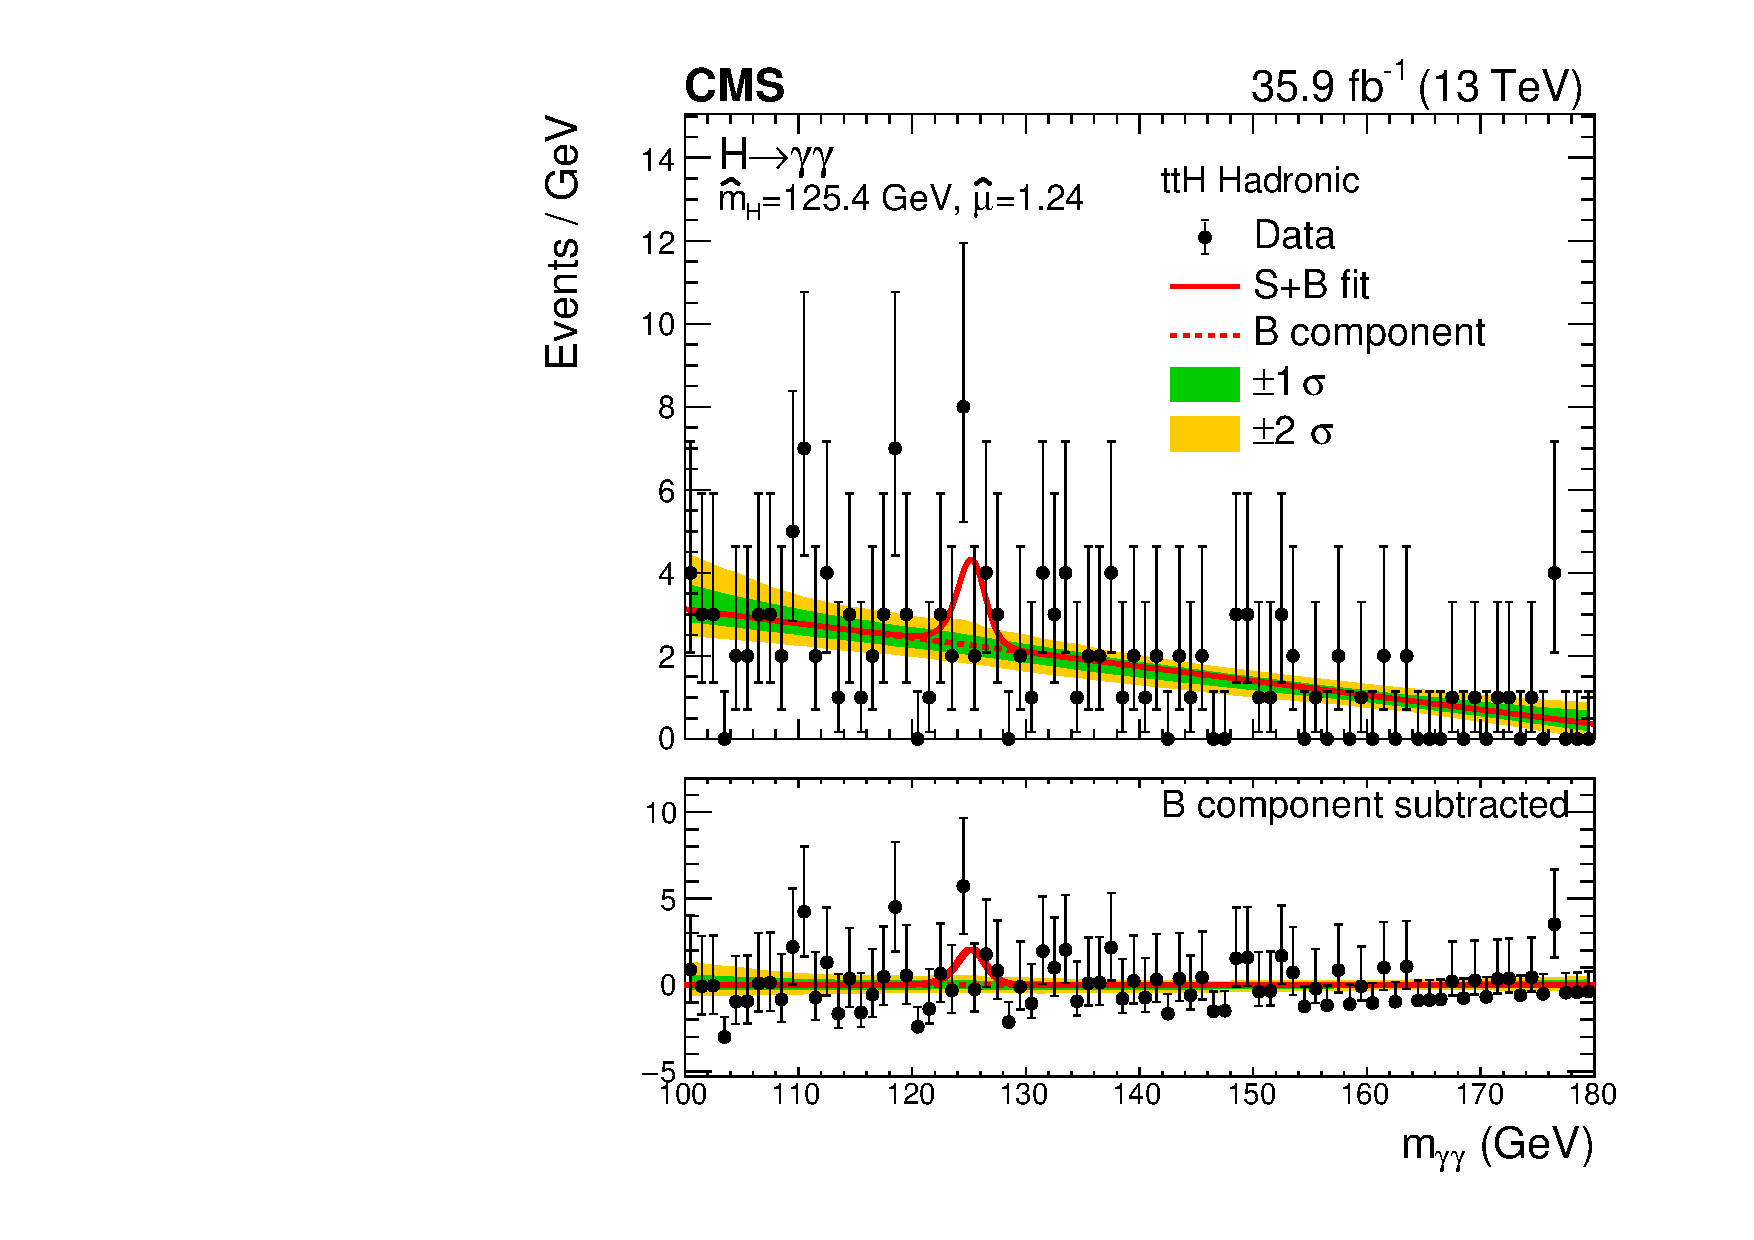
\includegraphics[width=0.47\textwidth]{figures/appendix_mass_plots/SBplots_jackWSnewOldTTHTTHHadronicTag_13TeV.pdf}
    \end{center}
    \label{fig:app_mass_plots:tth}
    \caption{Mass plots of the \ttH tags. BDT-based VBF analysis is on the left and DCNN-based is on the right.}
\end{figure}

\begin{figure}[h!]
    \begin{center}
        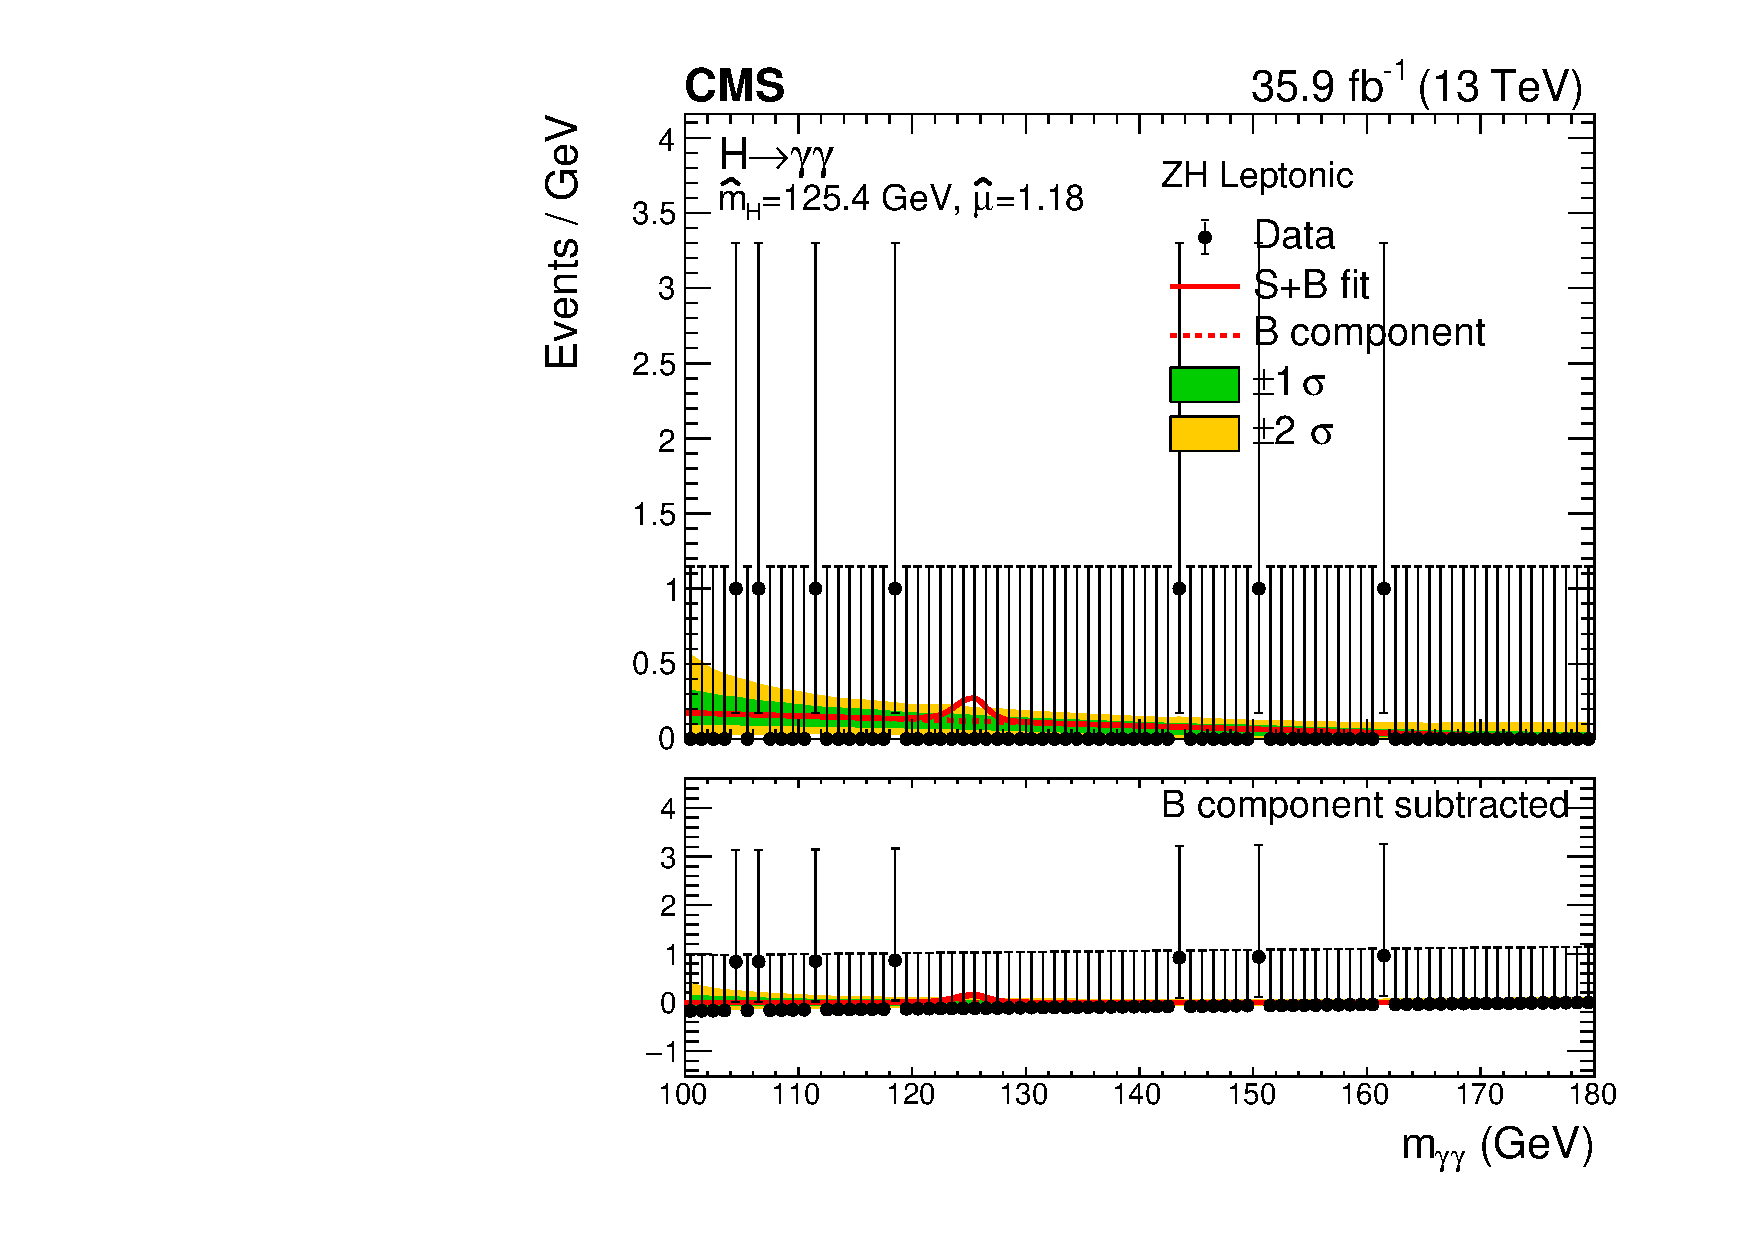
\includegraphics[width=0.47\textwidth]{figures/appendix_mass_plots/CMS-HIG-16-040_Figure_013-a.pdf}
        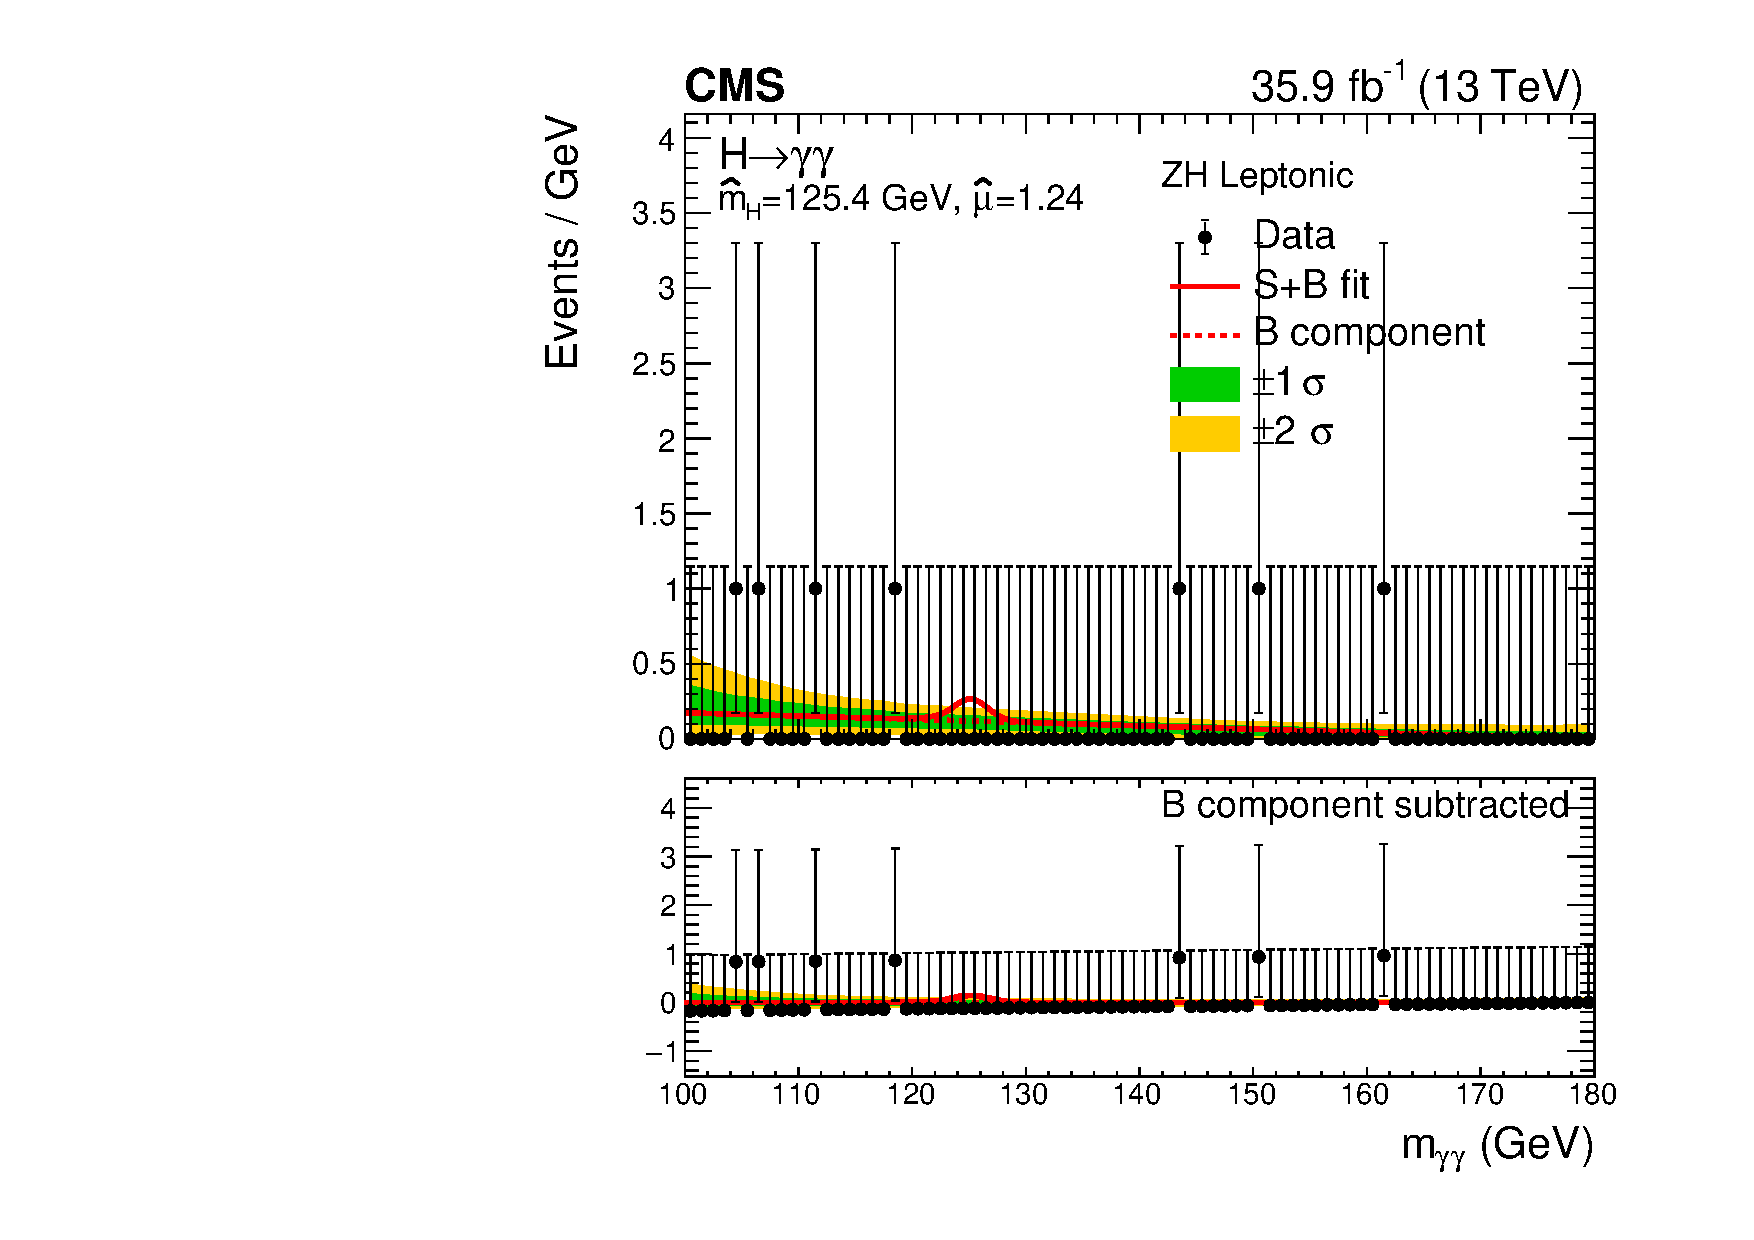
\includegraphics[width=0.47\textwidth]{figures/appendix_mass_plots/SBplots_jackWSnewOldTTHZHLeptonicTag_13TeV.pdf}
    \end{center}
    \begin{center}
        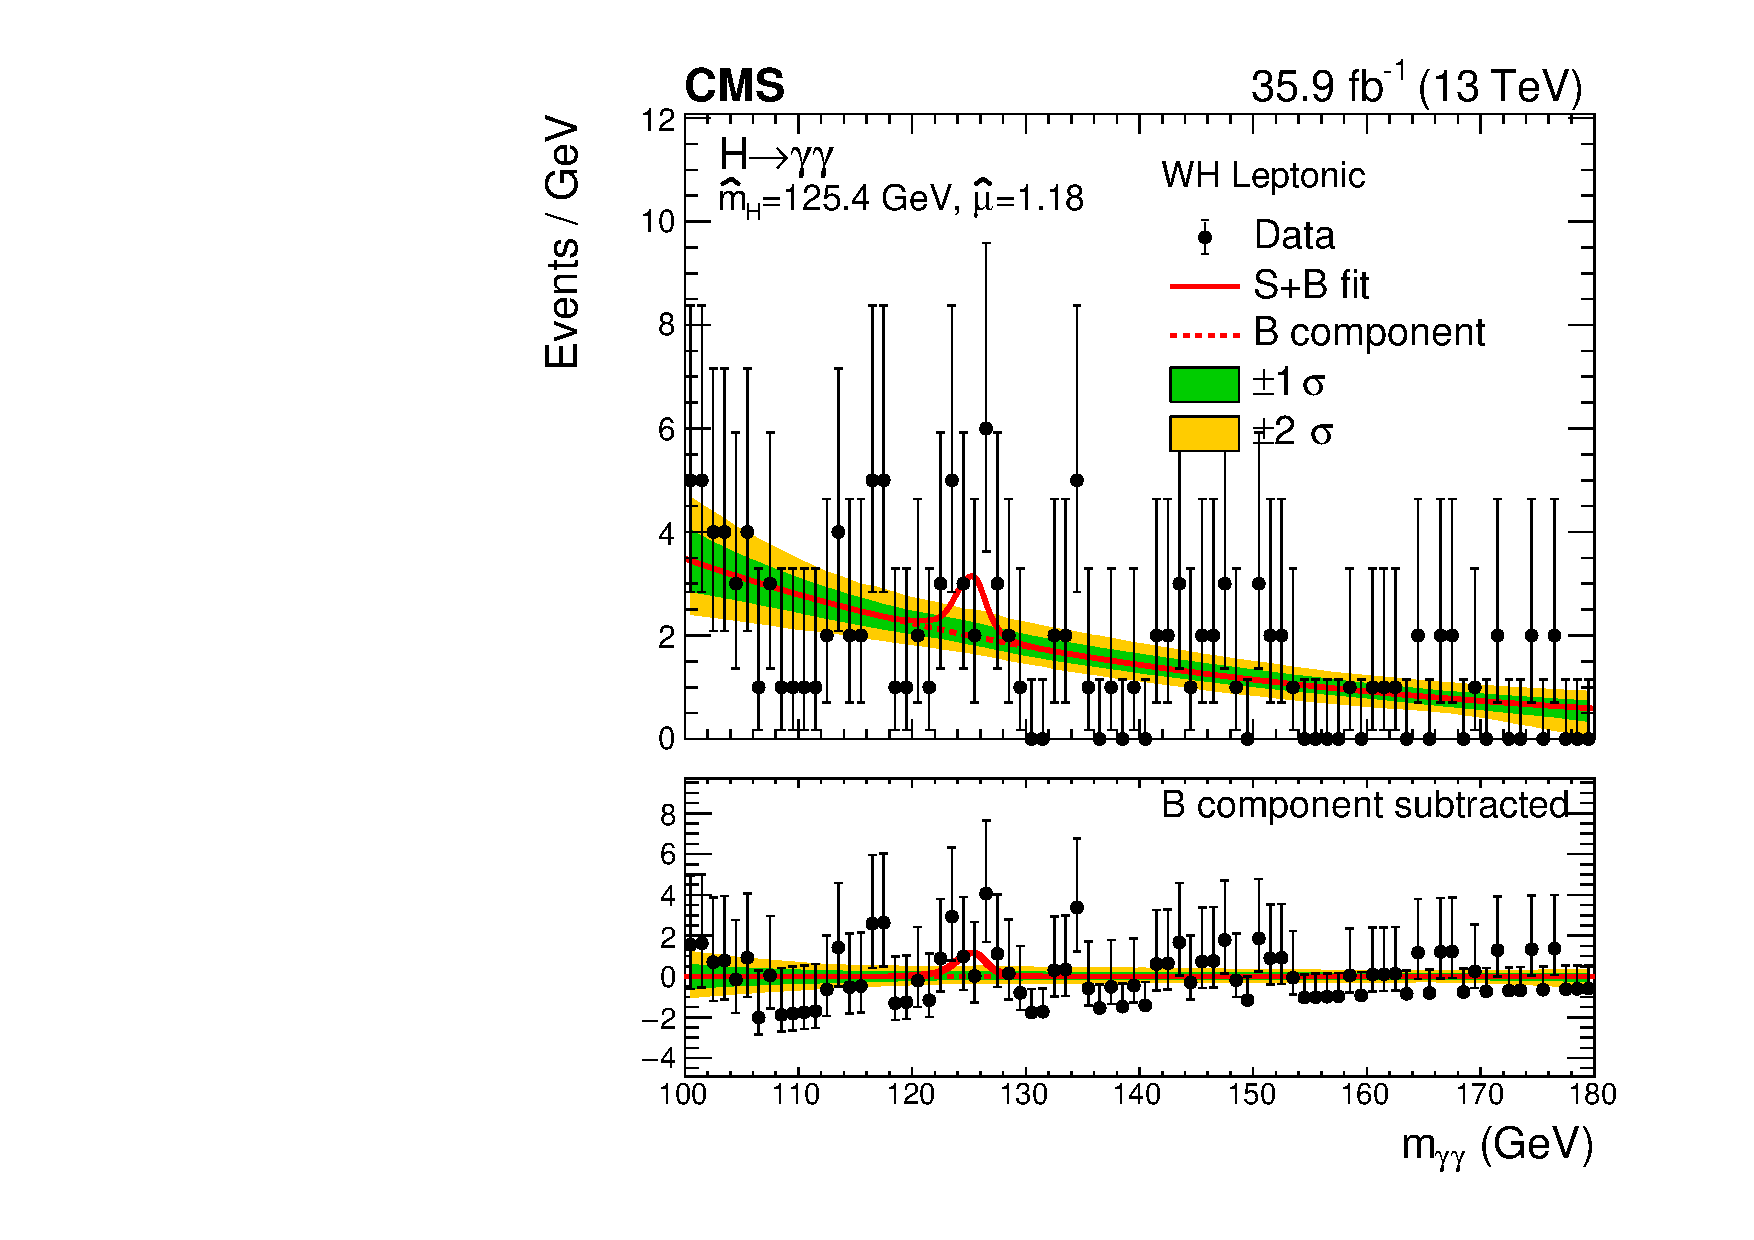
\includegraphics[width=0.47\textwidth]{figures/appendix_mass_plots/CMS-HIG-16-040_Figure_013-b.pdf}
        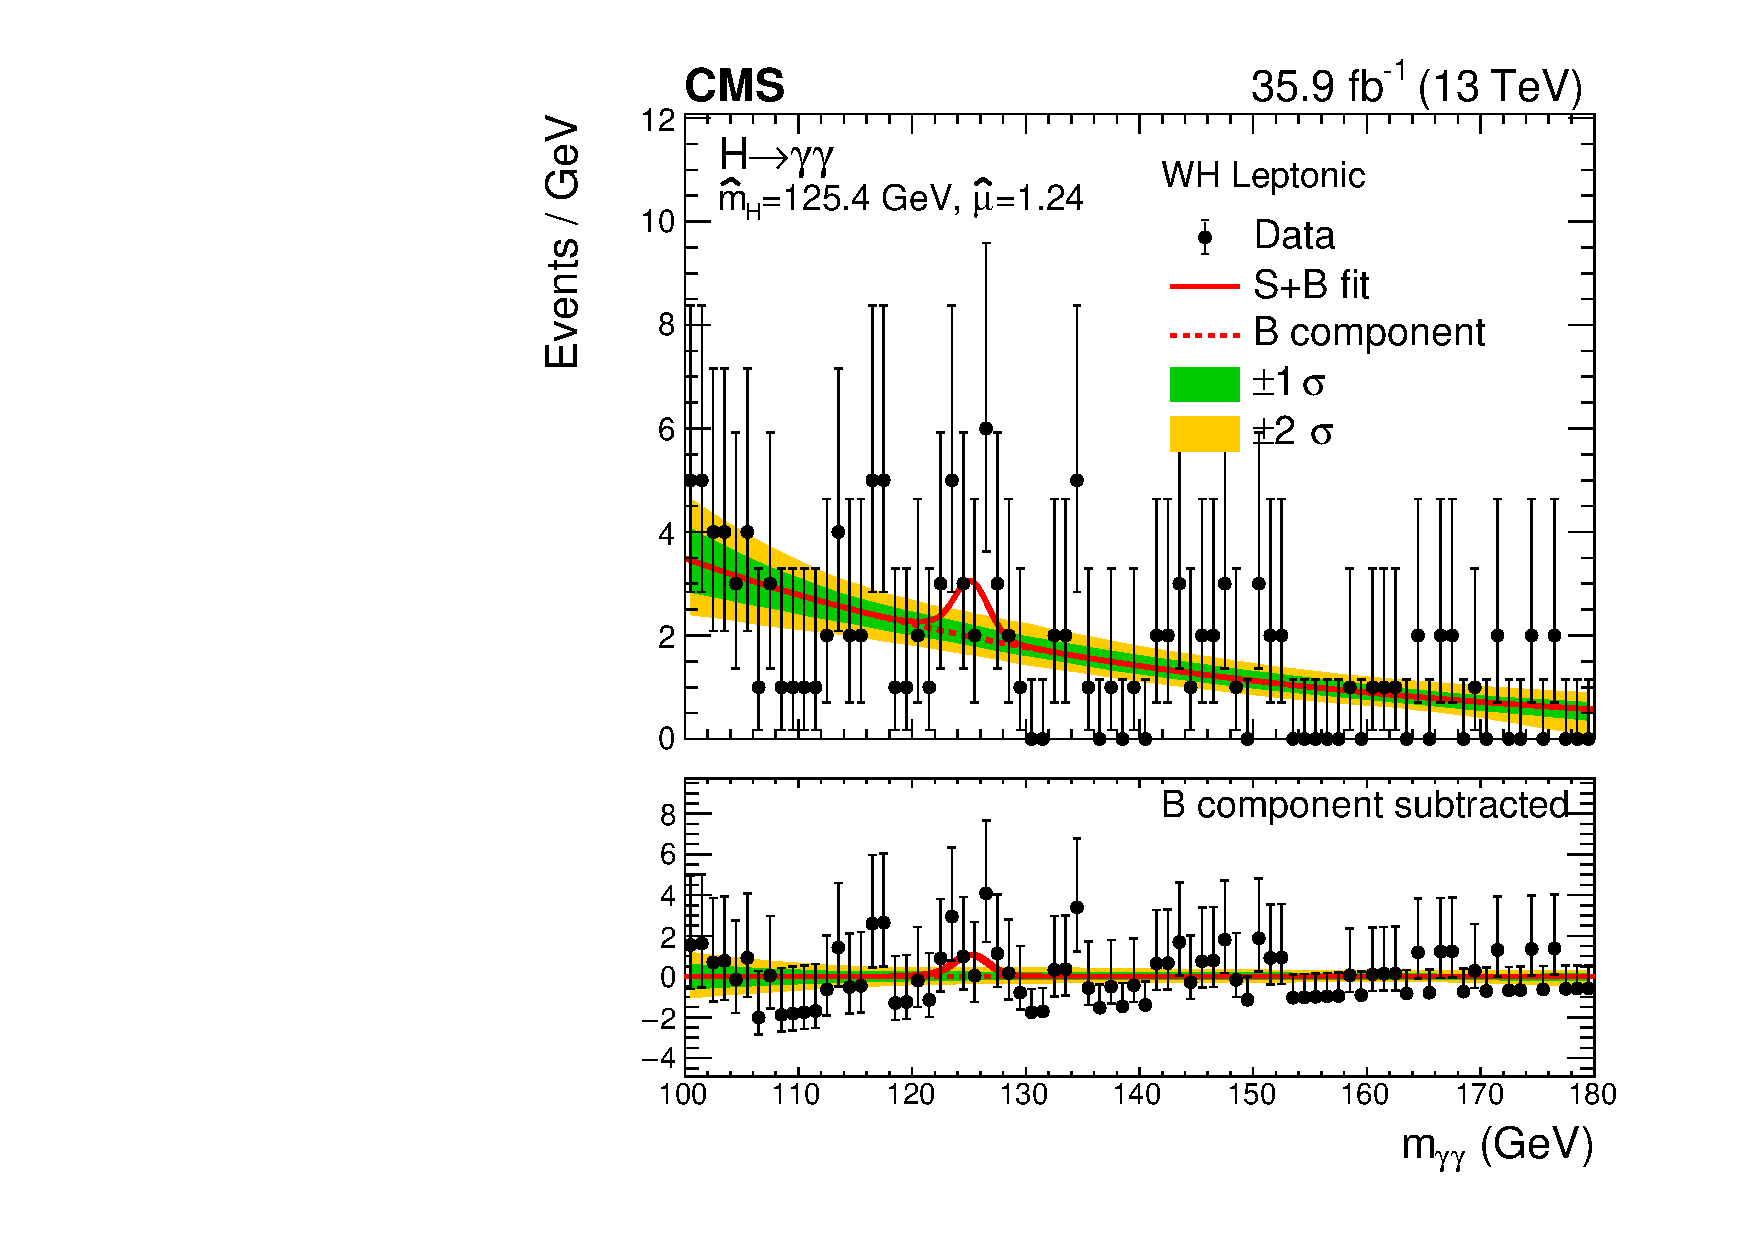
\includegraphics[width=0.47\textwidth]{figures/appendix_mass_plots/SBplots_jackWSnewOldTTHWHLeptonicTag_13TeV.pdf}
    \end{center}
    \begin{center}
        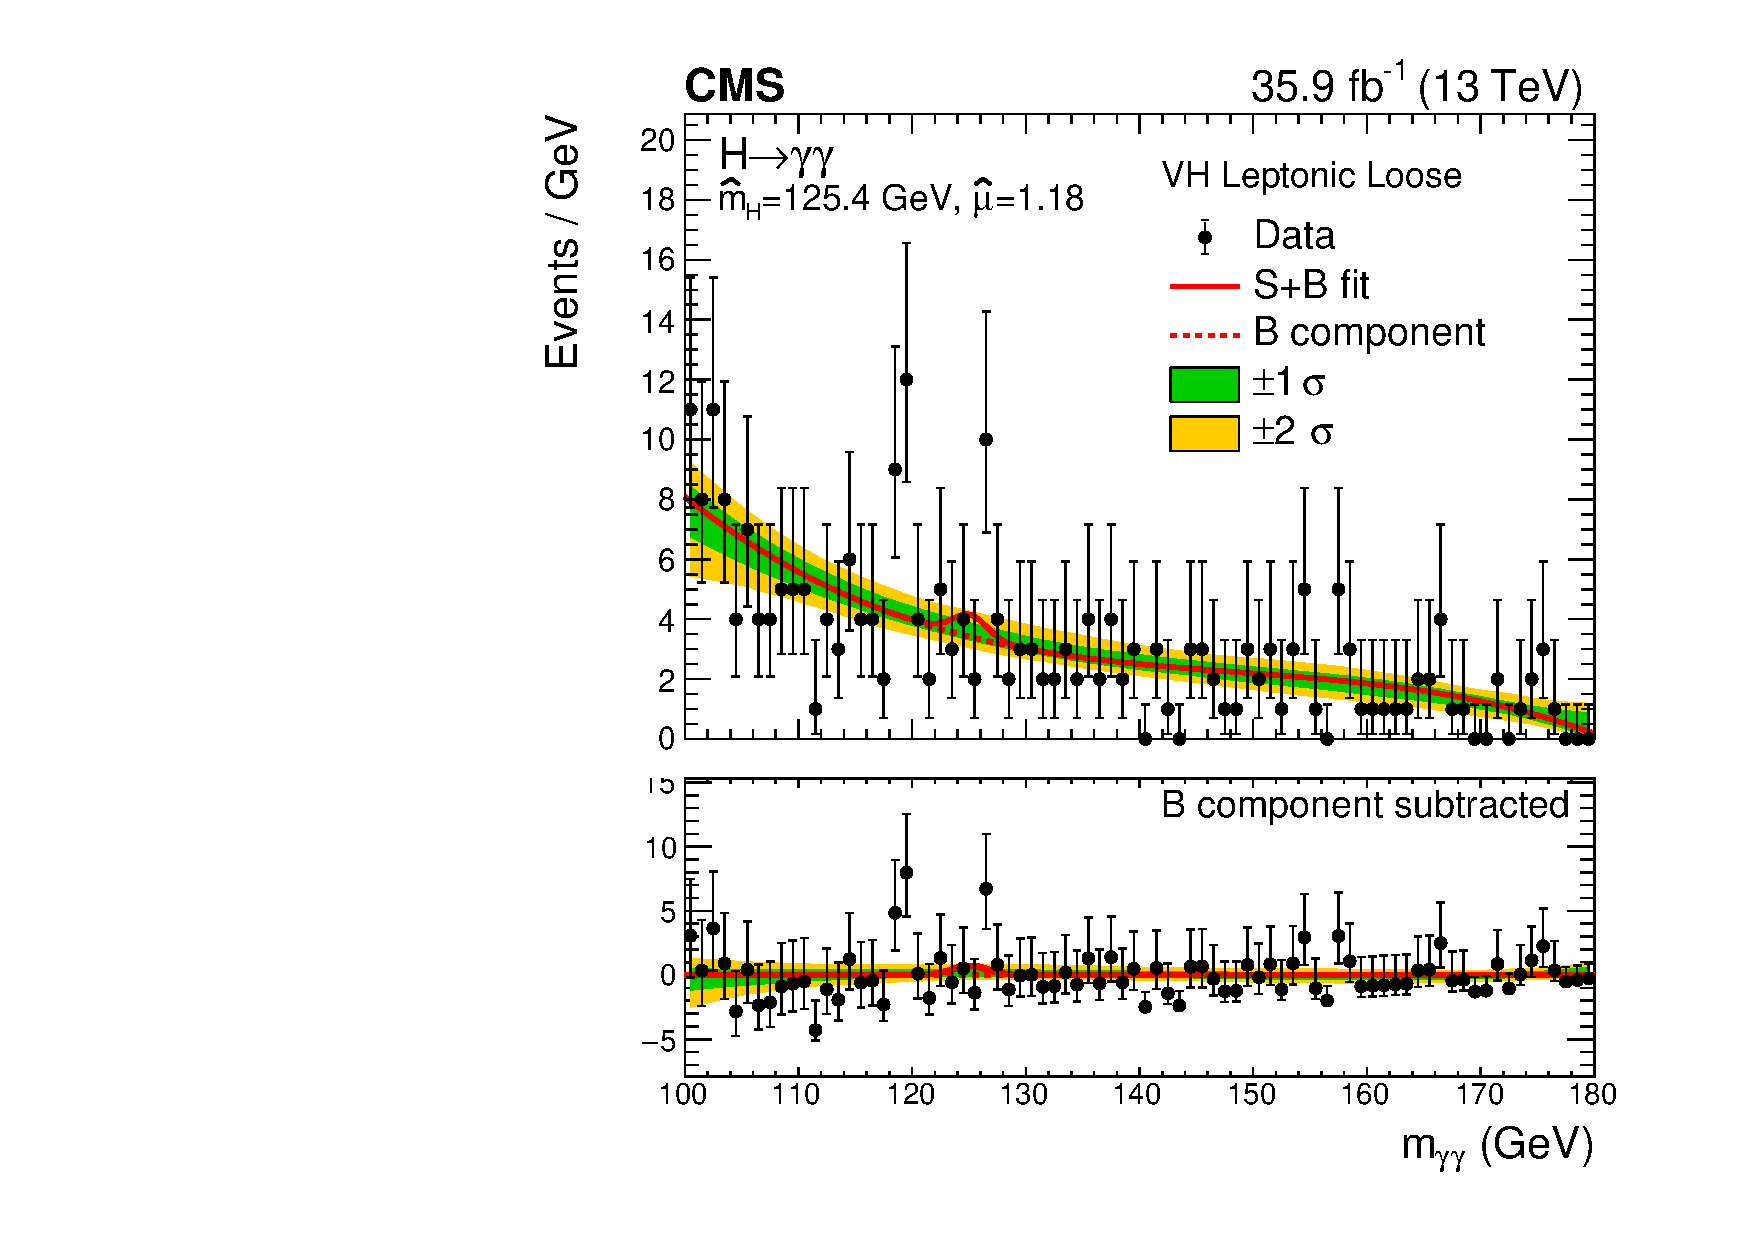
\includegraphics[width=0.47\textwidth]{figures/appendix_mass_plots/CMS-HIG-16-040_Figure_013-c.pdf}
        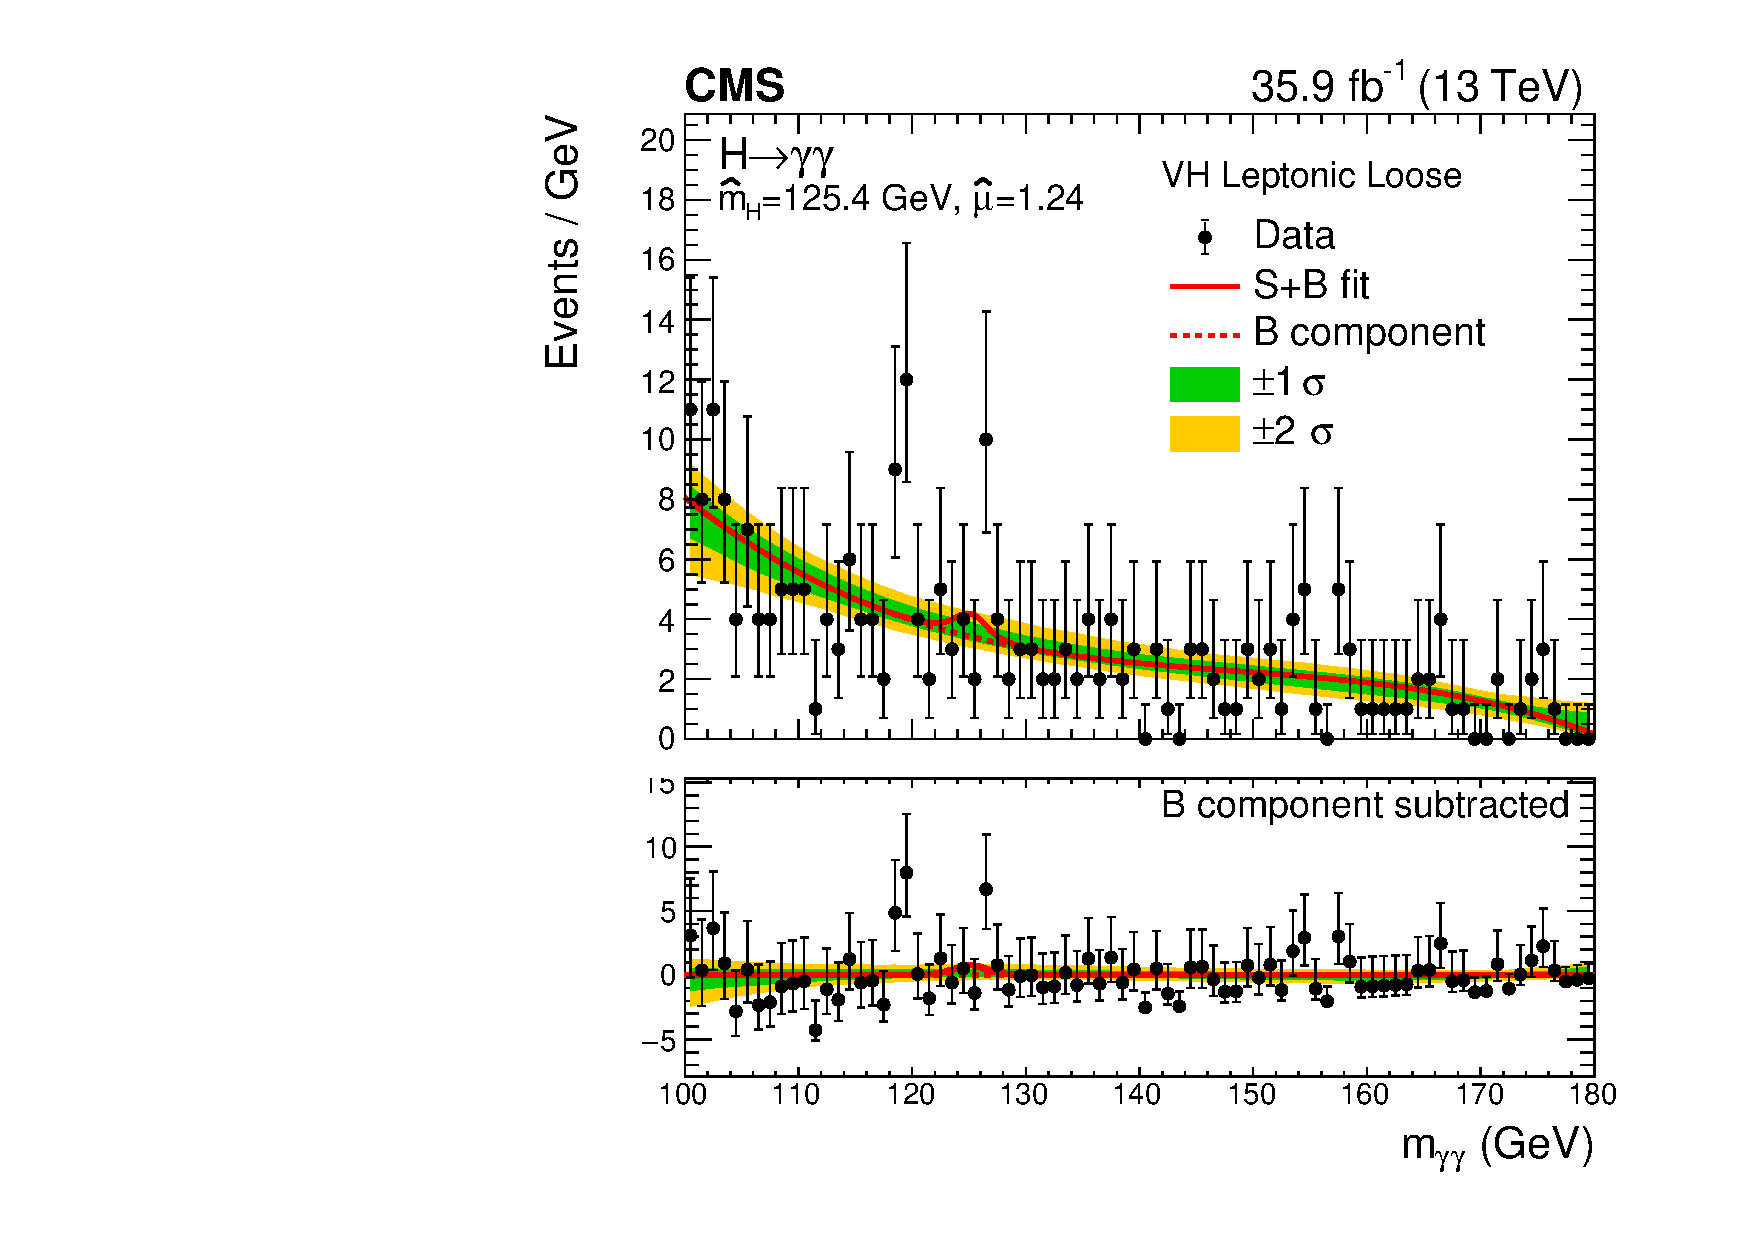
\includegraphics[width=0.47\textwidth]{figures/appendix_mass_plots/SBplots_jackWSnewOldTTHVHLeptonicLooseTag_13TeV.pdf}
    \end{center}
    \label{fig:app_mass_plots:vh_lep}
    \caption{VH leptonic tags. BDT-based VBF analysis is on the left and DCNN-based is on the right.}
\end{figure}

\begin{figure}[h!]
    \begin{center}
        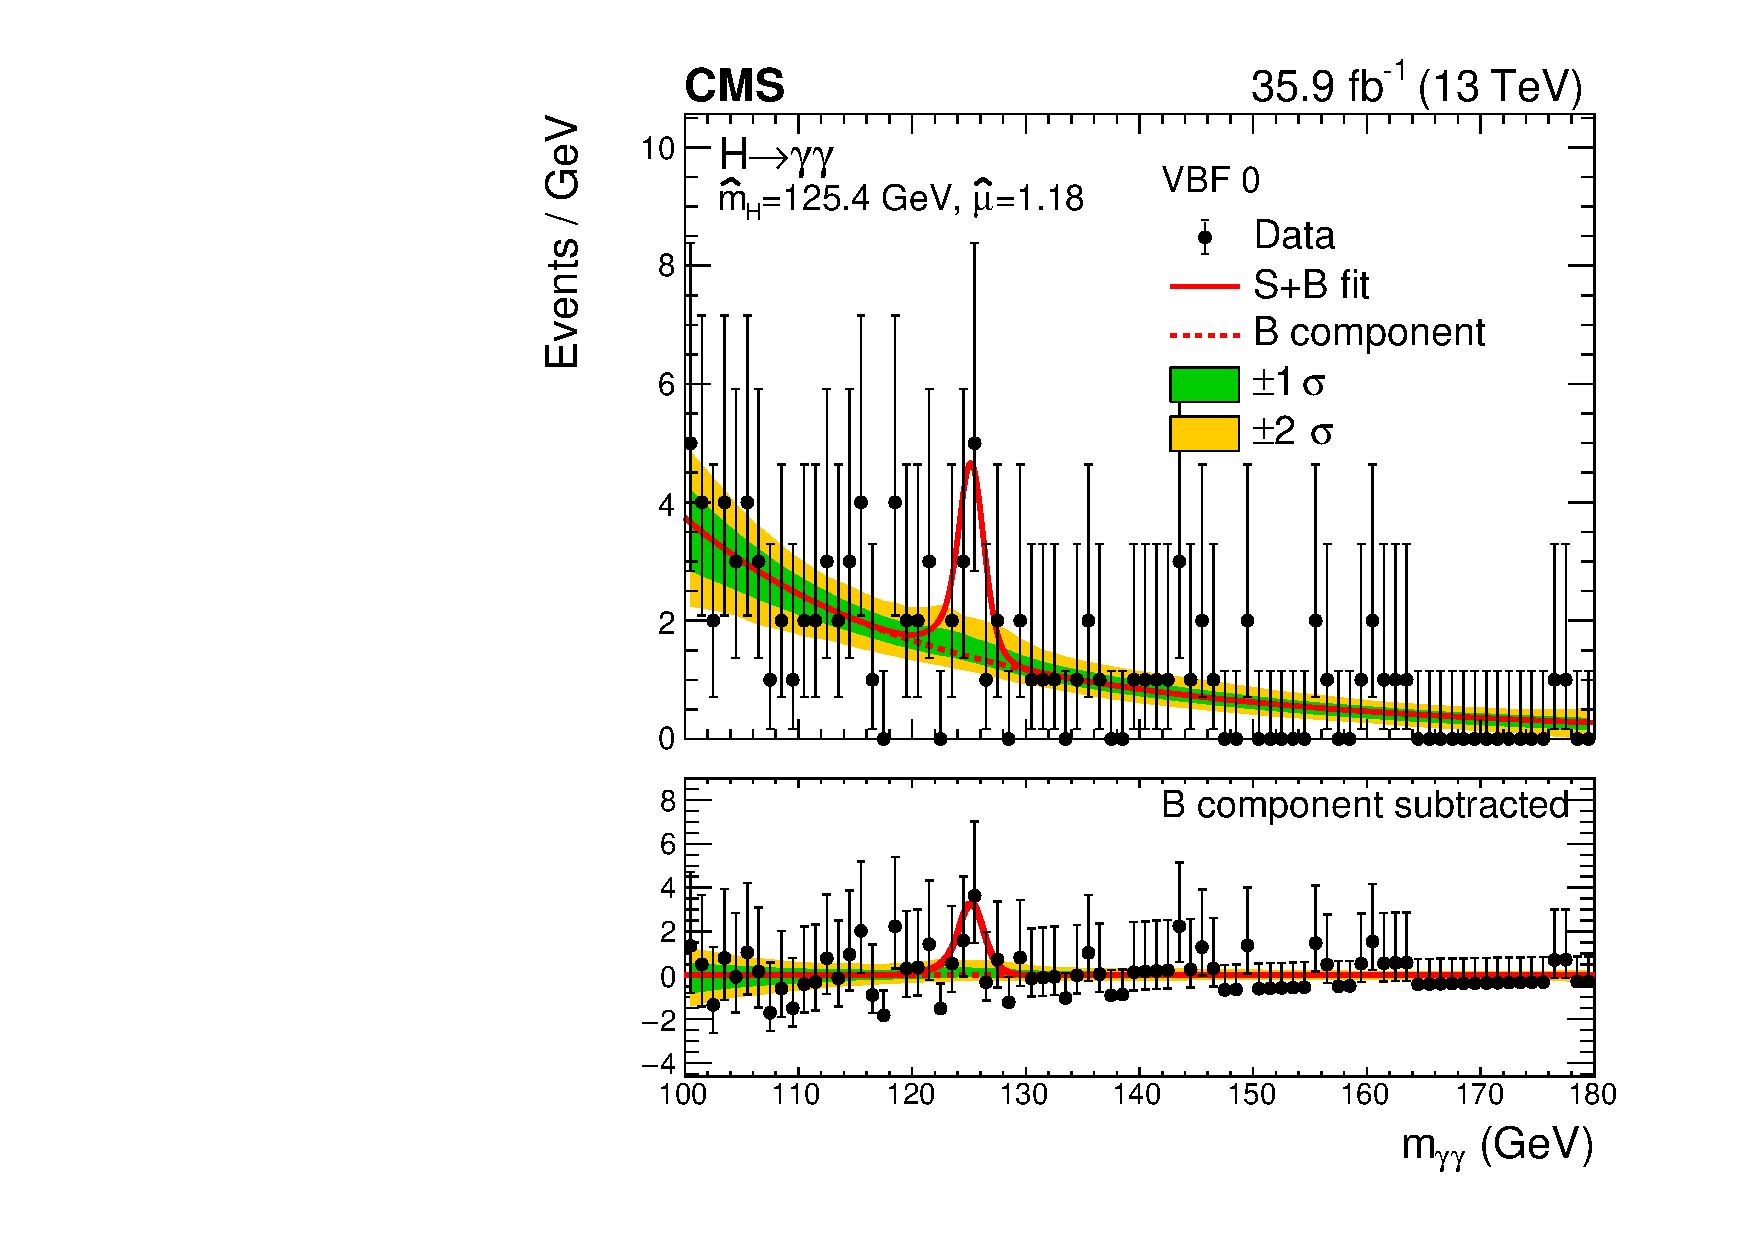
\includegraphics[width=0.47\textwidth]{figures/stats_results/CMS-HIG-16-040_Figure_012-a.pdf}
        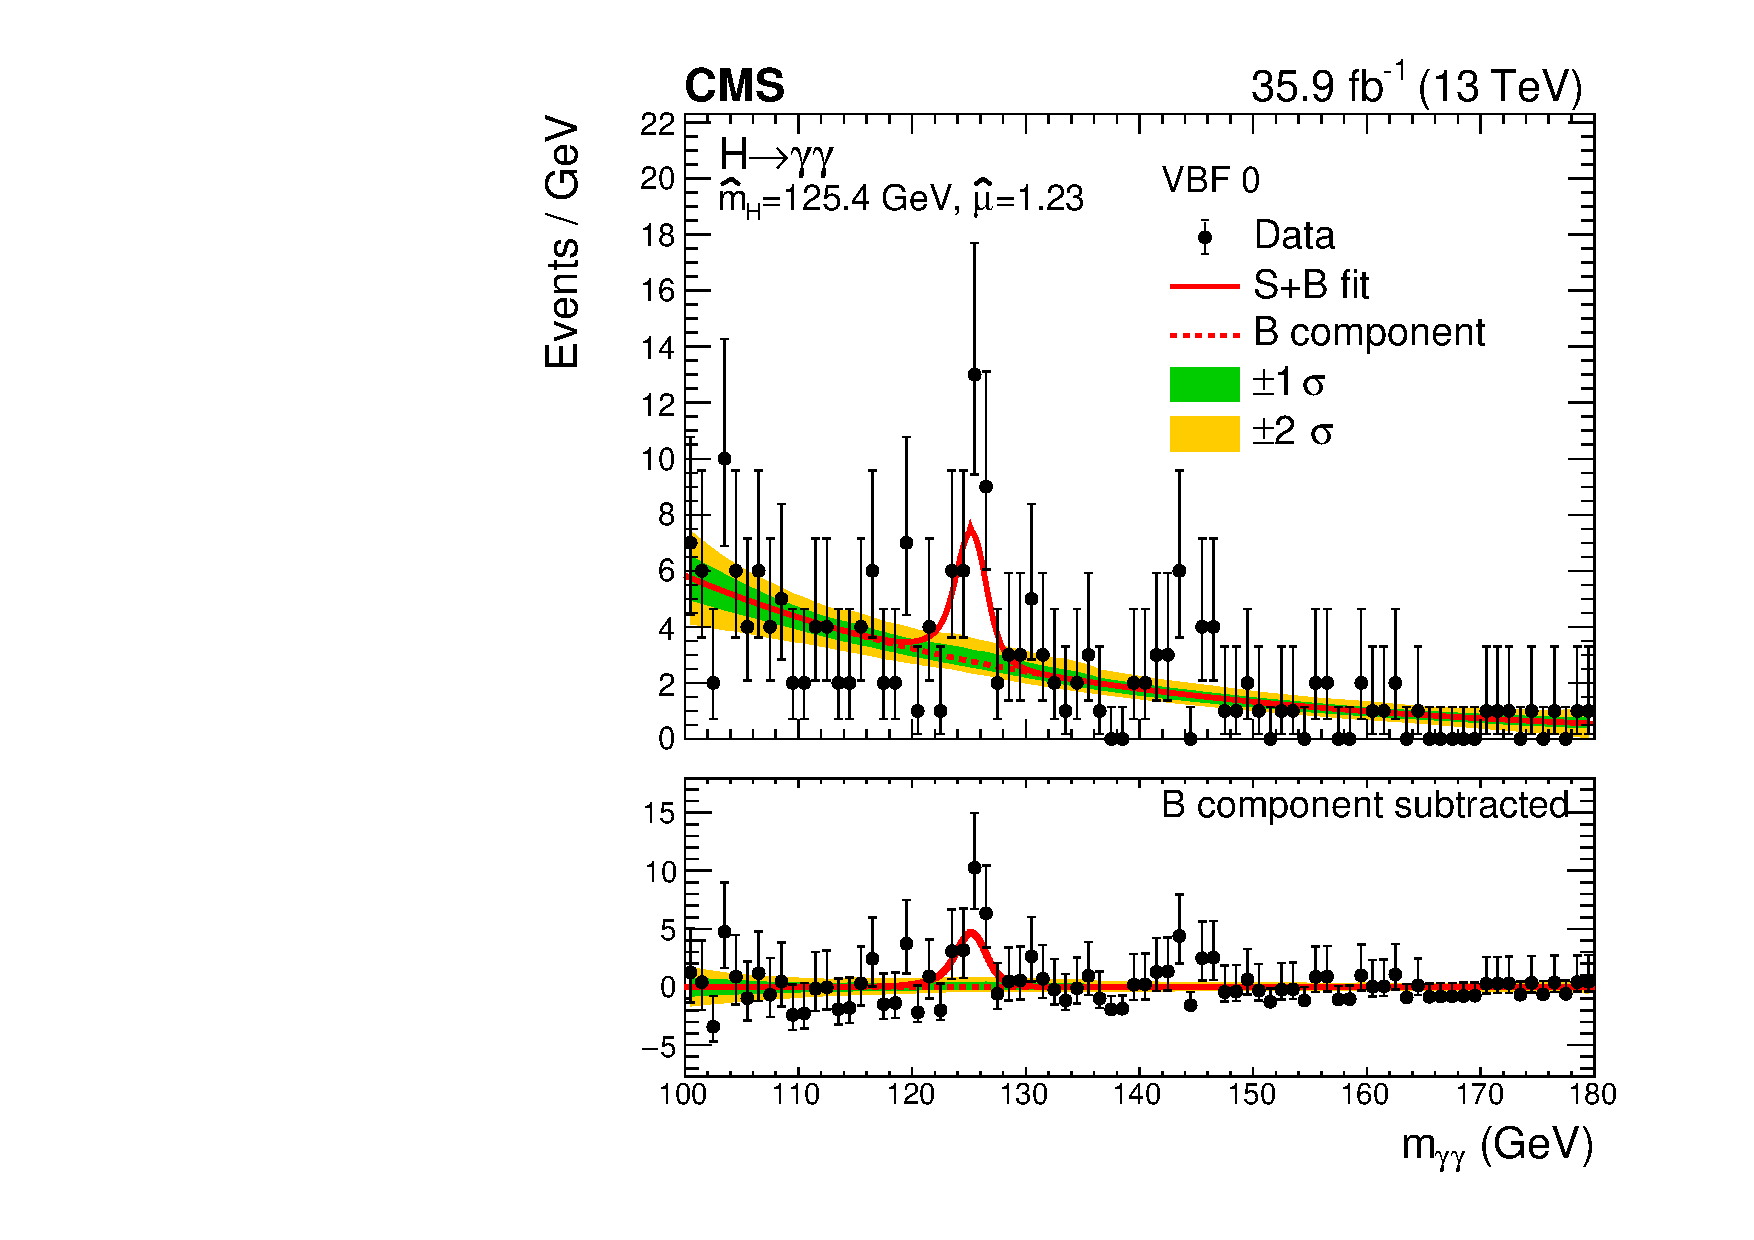
\includegraphics[width=0.47\textwidth]{figures/stats_results/SBplots_jackWSnewVBFTag_0_13TeV.pdf}
    \end{center}
    \begin{center}
        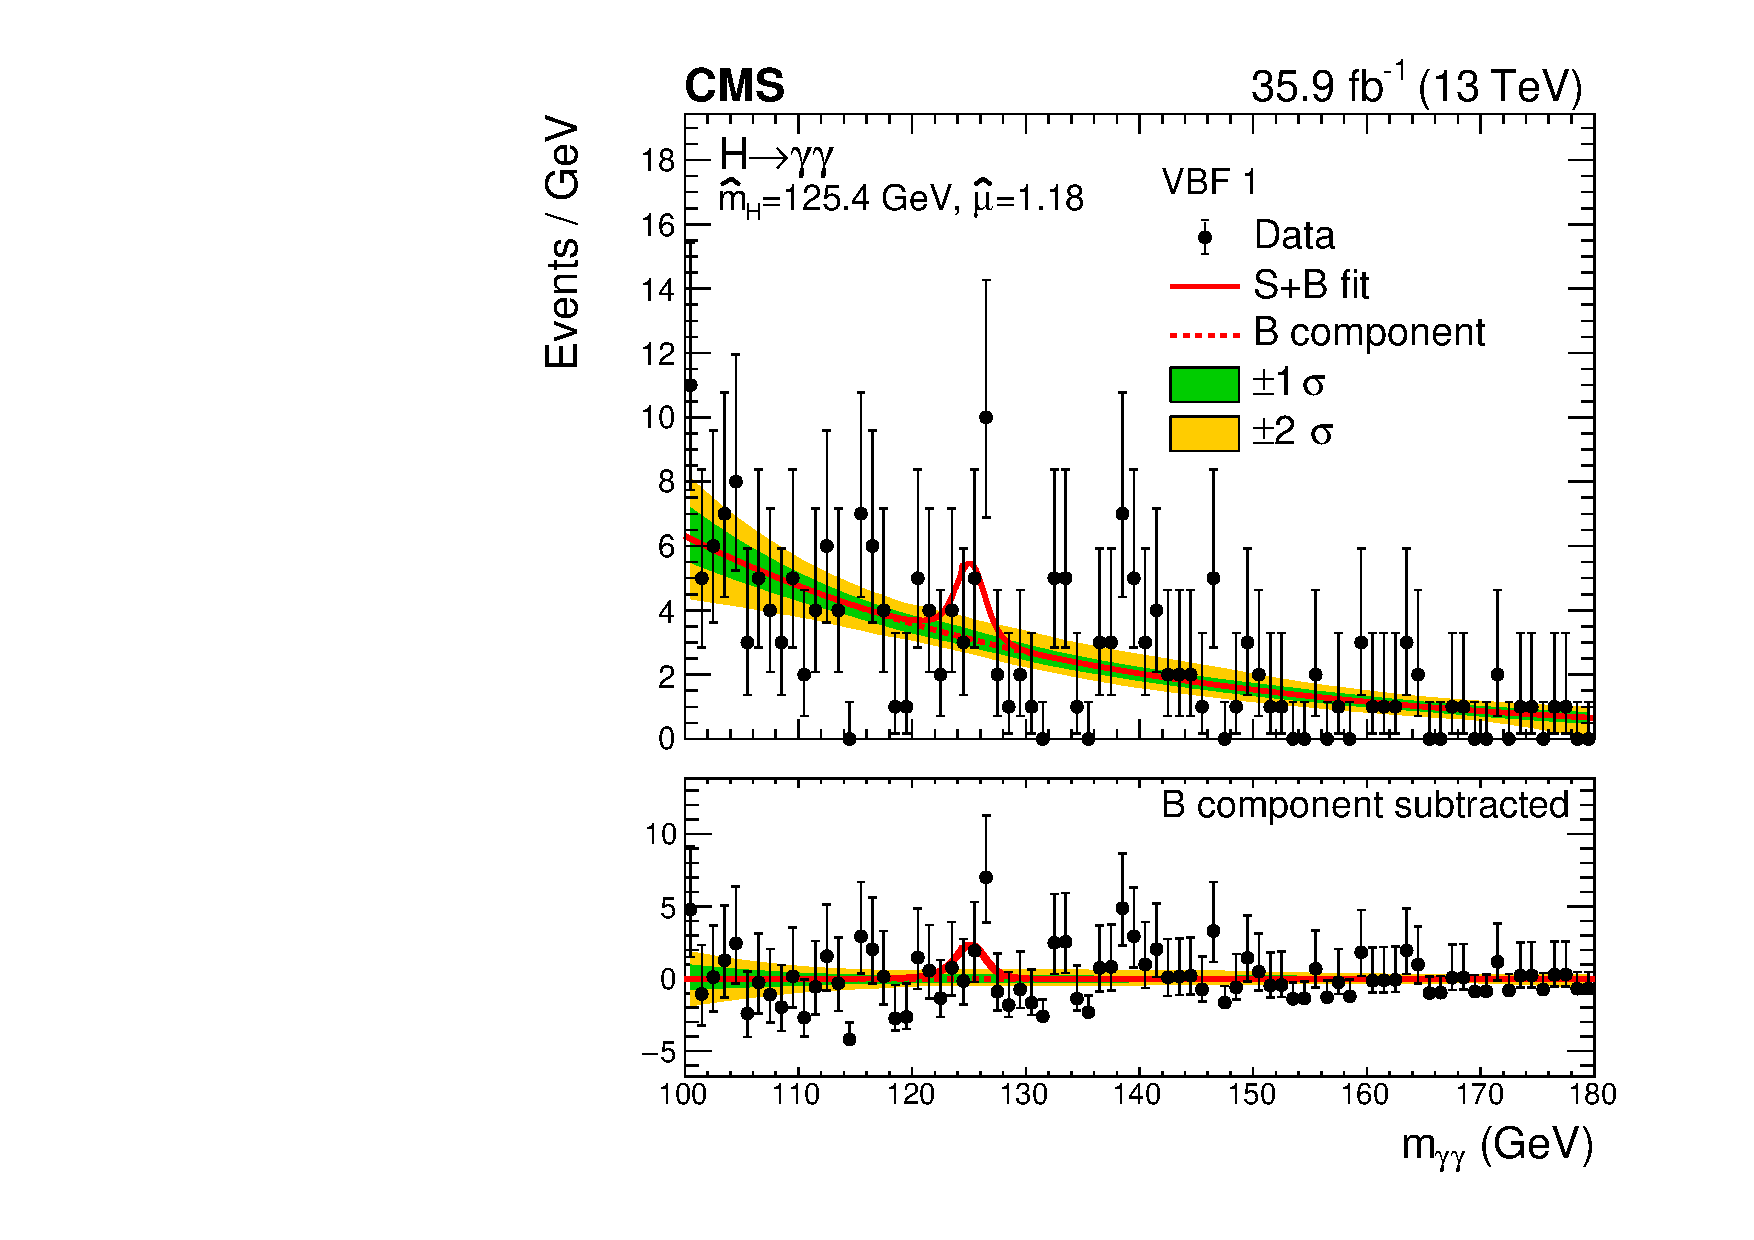
\includegraphics[width=0.47\textwidth]{figures/stats_results/CMS-HIG-16-040_Figure_012-b.pdf}
        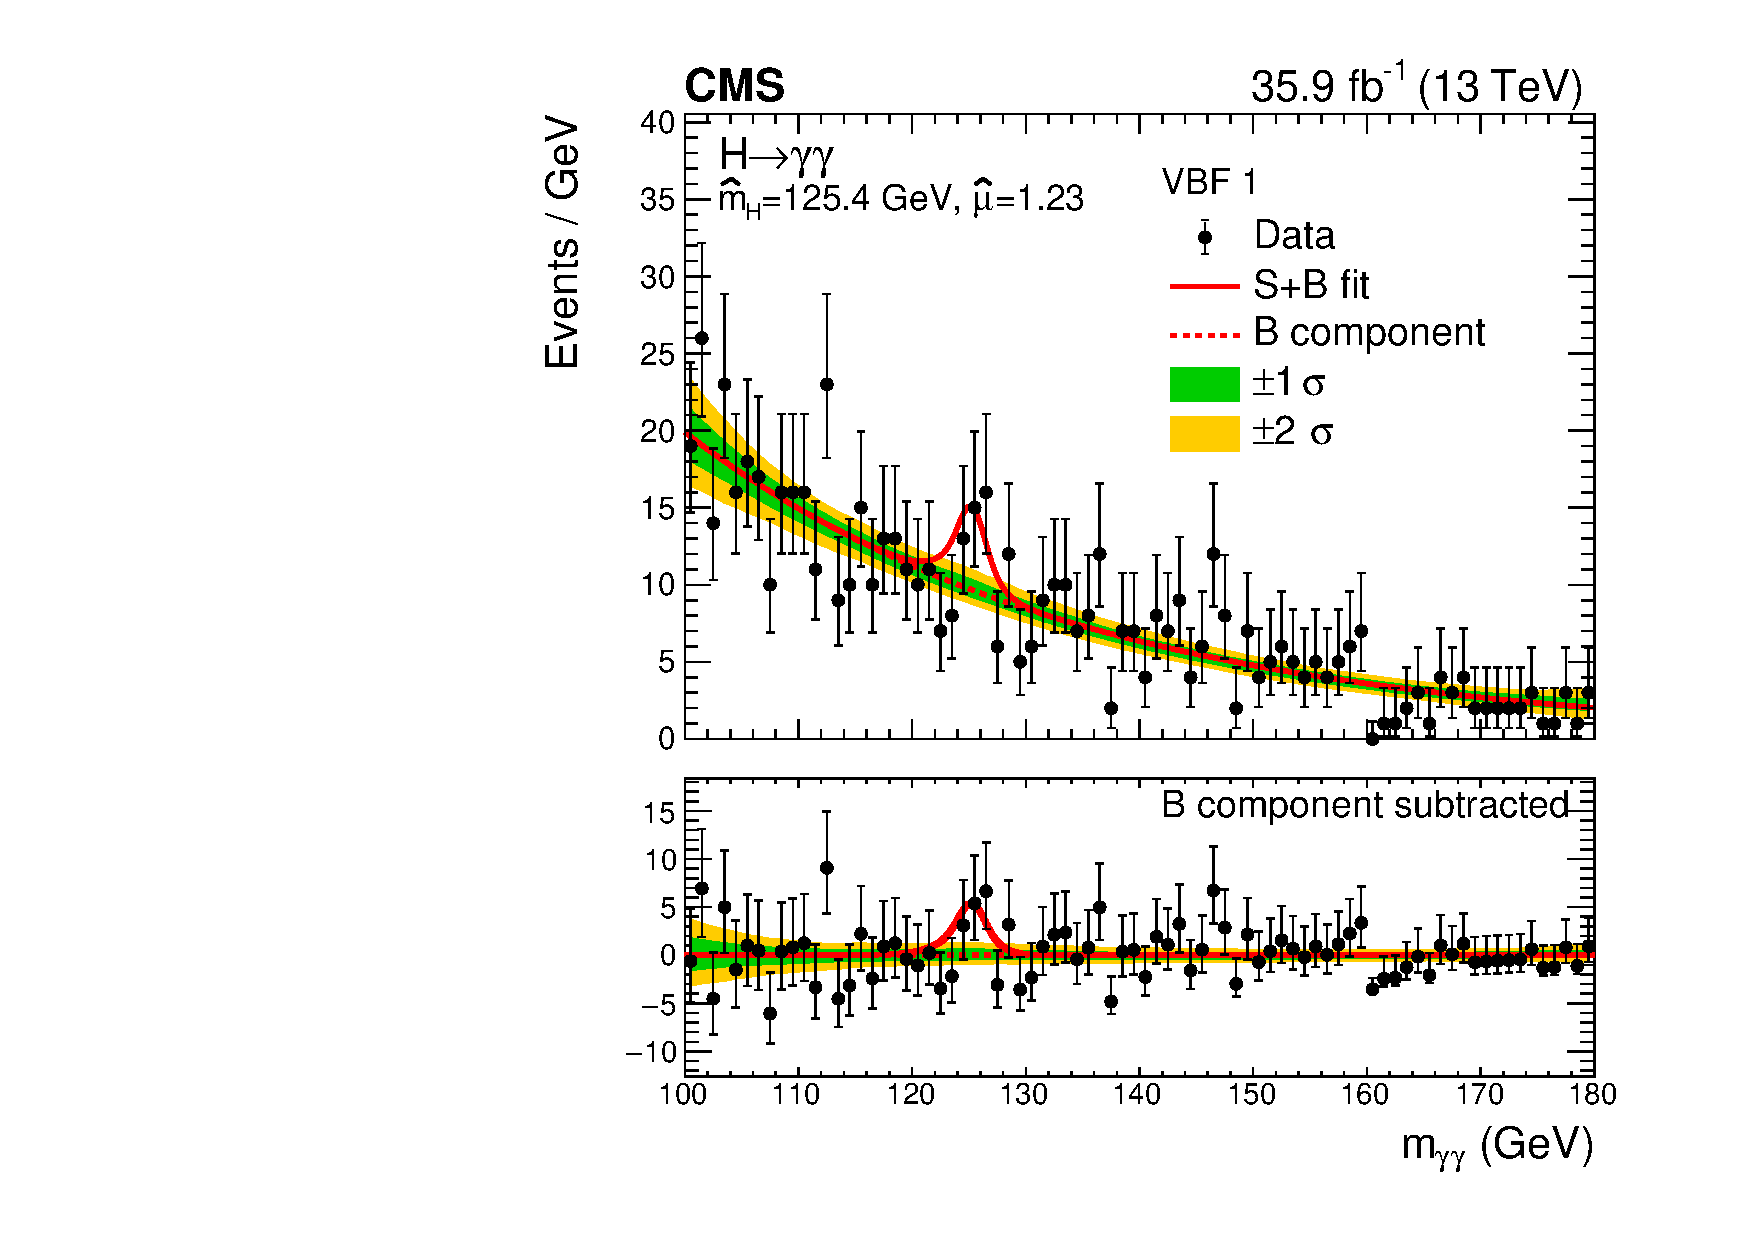
\includegraphics[width=0.47\textwidth]{figures/stats_results/SBplots_jackWSnewVBFTag_1_13TeV.pdf}
    \end{center}
    \begin{center}
        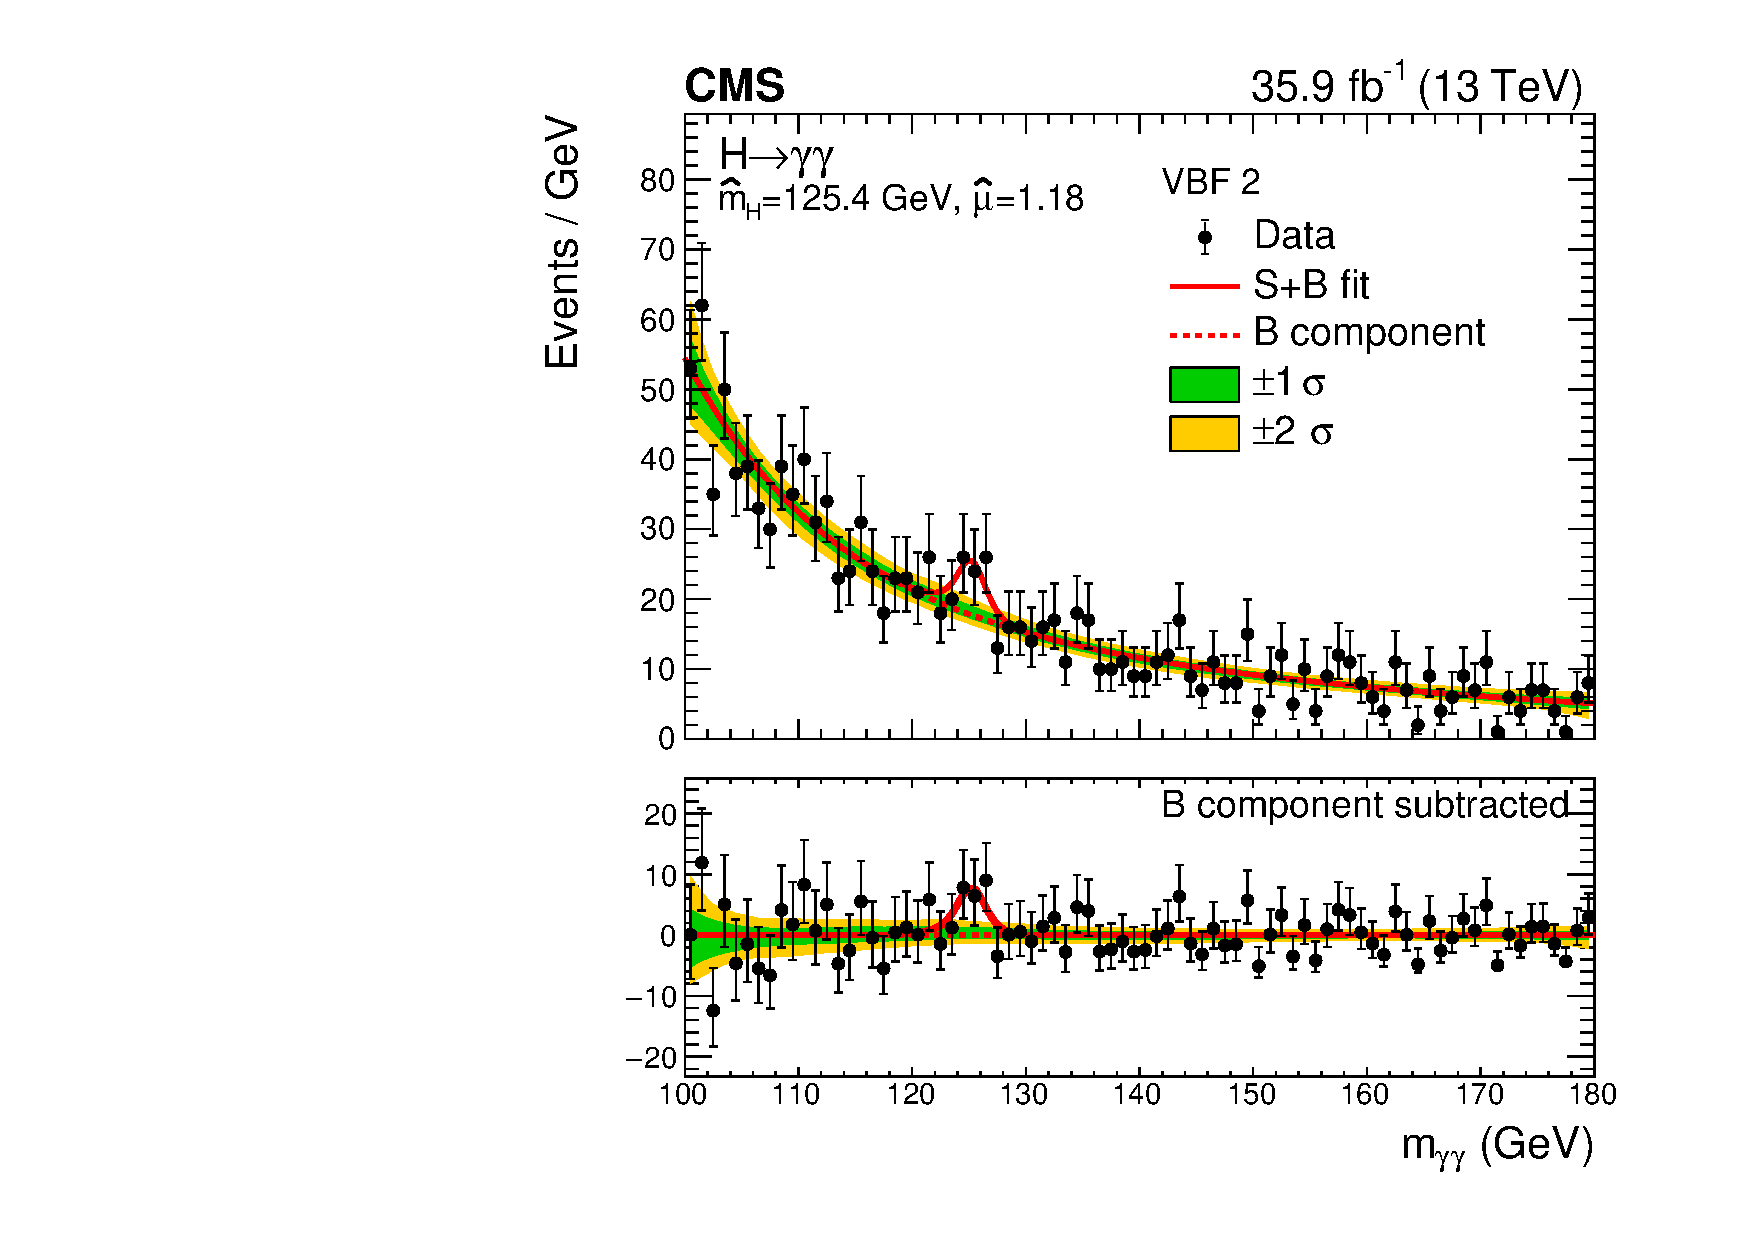
\includegraphics[width=0.47\textwidth]{figures/stats_results/CMS-HIG-16-040_Figure_012-c.pdf}
        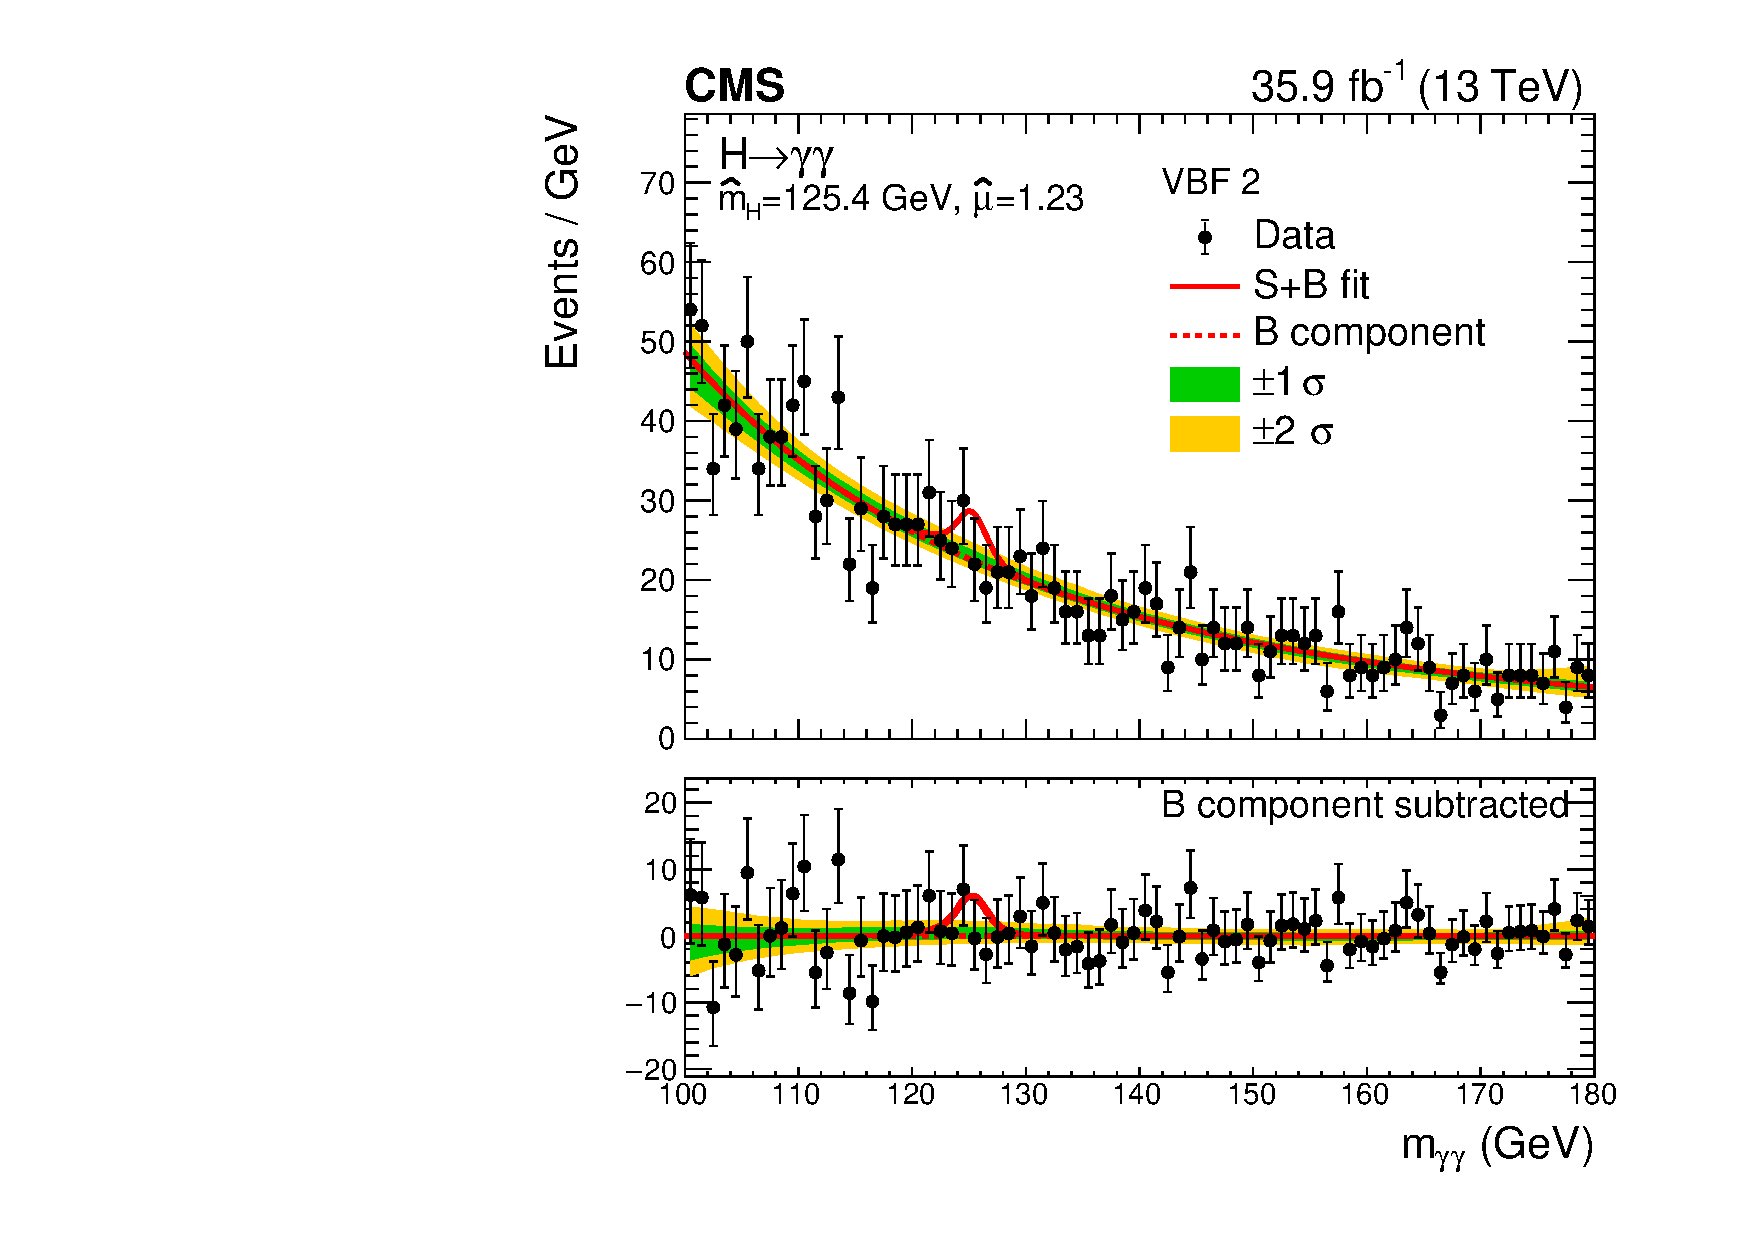
\includegraphics[width=0.47\textwidth]{figures/stats_results/SBplots_jackWSnewVBFTag_2_13TeV.pdf}
    \end{center}
    \caption{VBF tag categories. BDT-based VBF analysis is on the left and DCNN-based is on the right.}
        \label{fig:app_mass_plots:vbf}
\end{figure}

\begin{figure}[h!]
    \begin{center}
        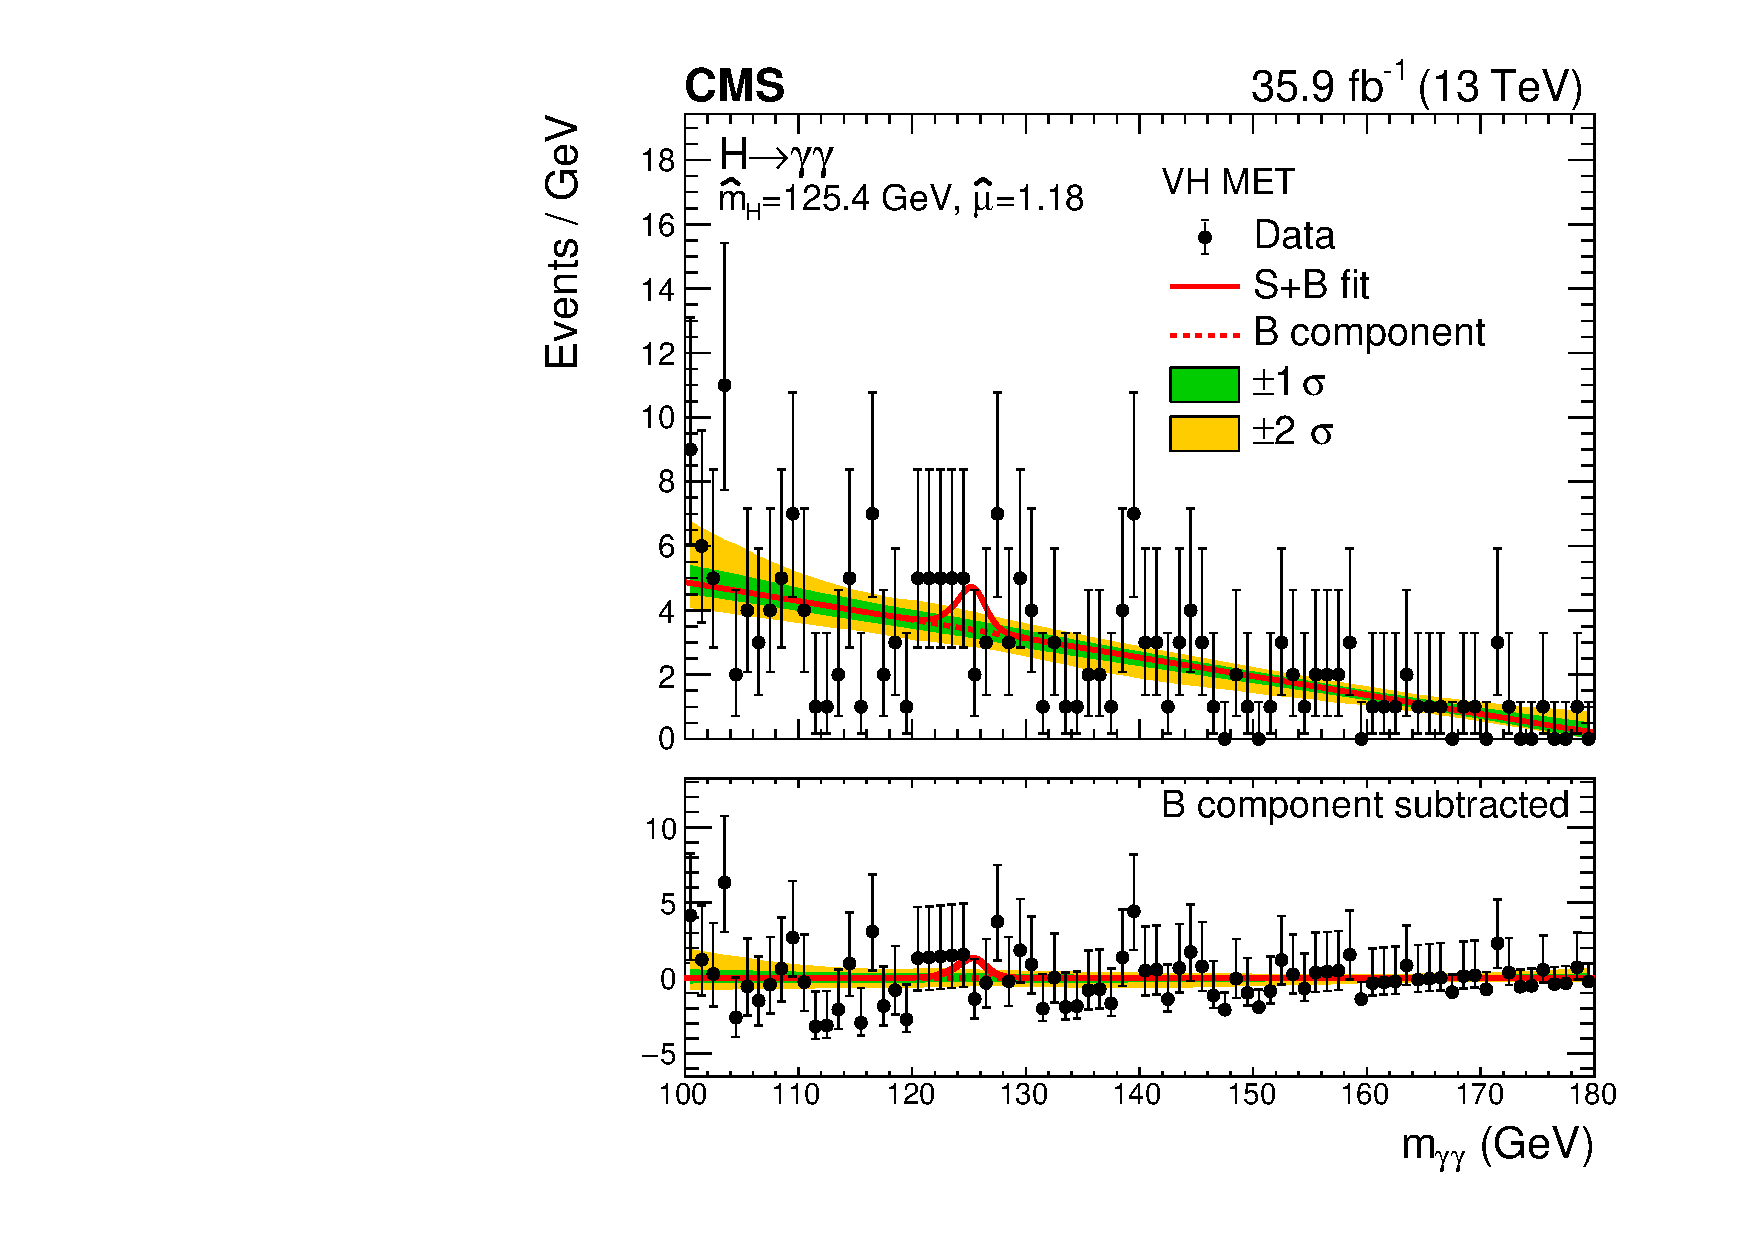
\includegraphics[width=0.47\textwidth]{figures/appendix_mass_plots/CMS-HIG-16-040_Figure_013-d.pdf}
        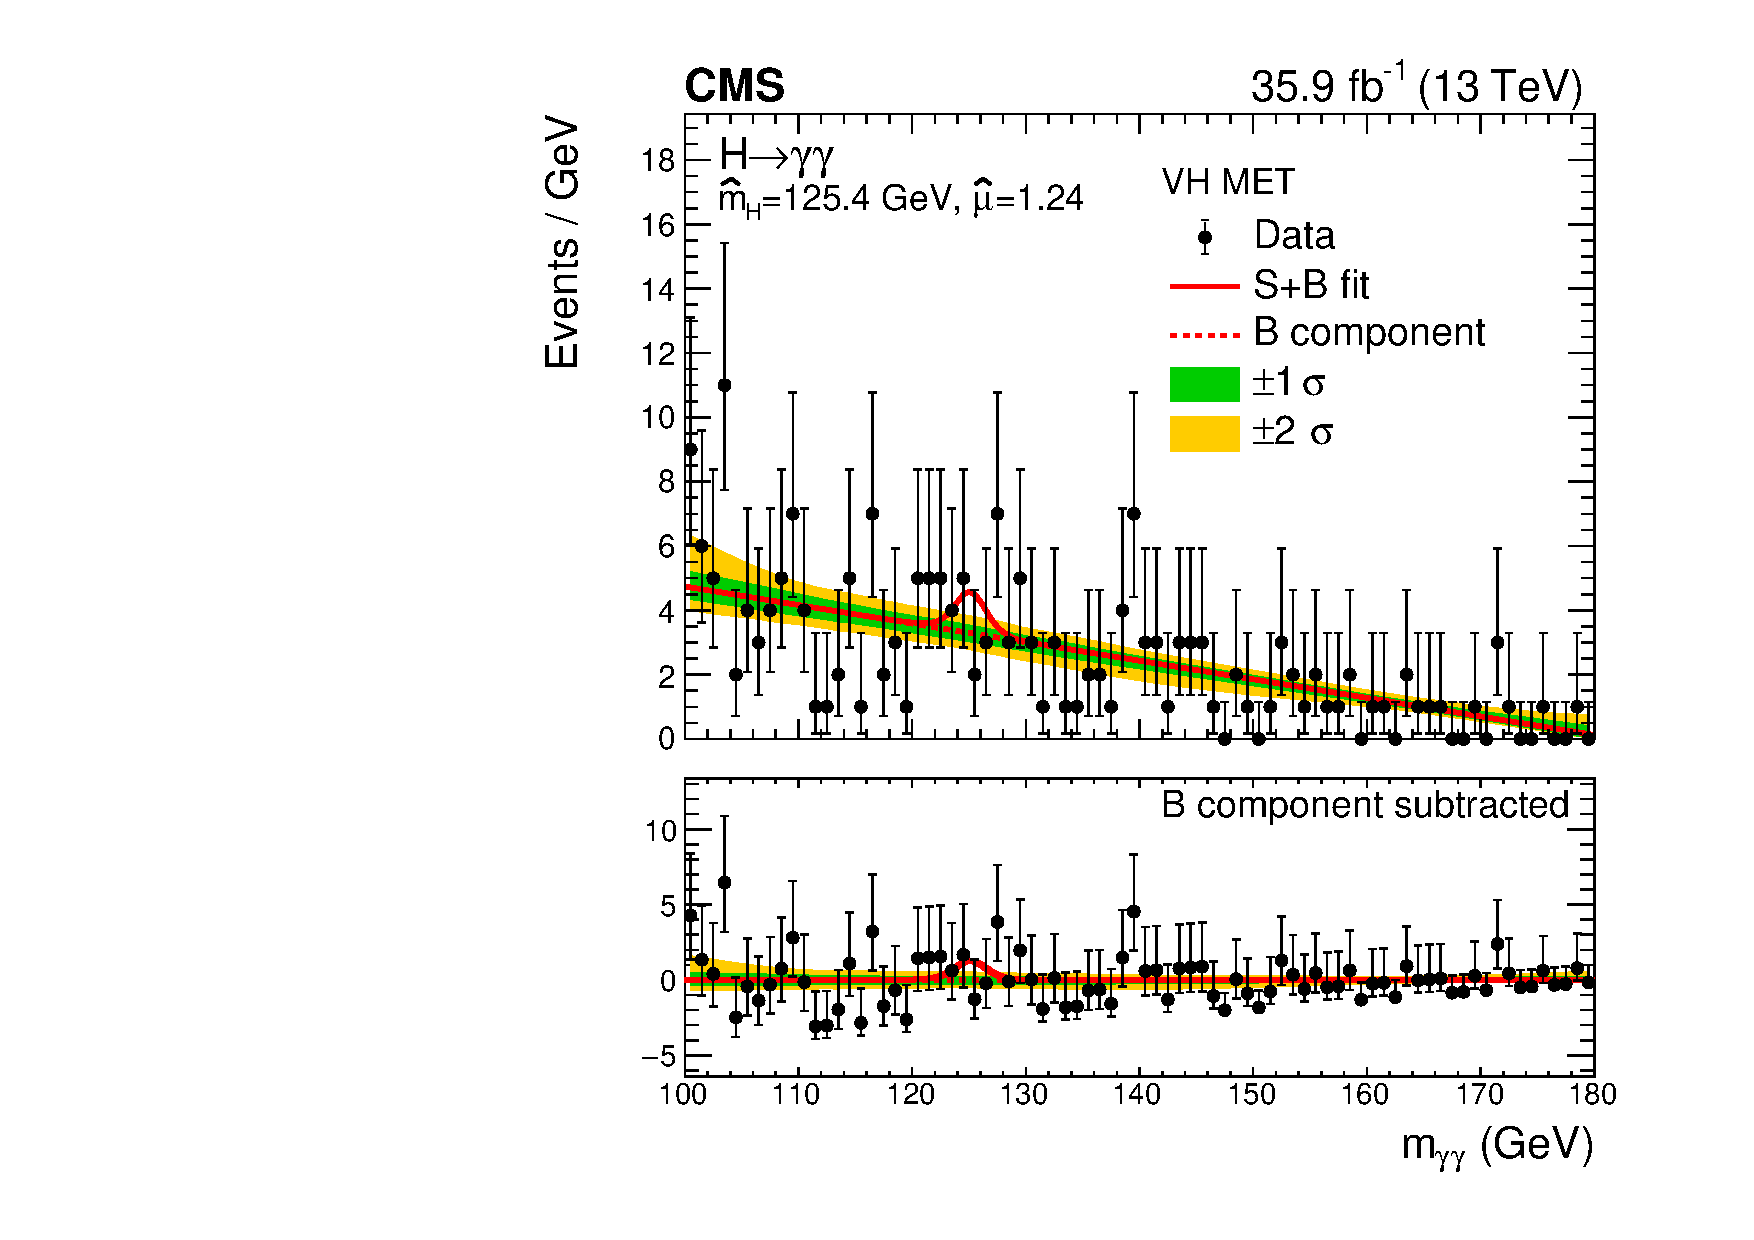
\includegraphics[width=0.47\textwidth]{figures/appendix_mass_plots/SBplots_jackWSnewOldTTHVHMetTag_13TeV.pdf}
    \end{center}
    \begin{center}
        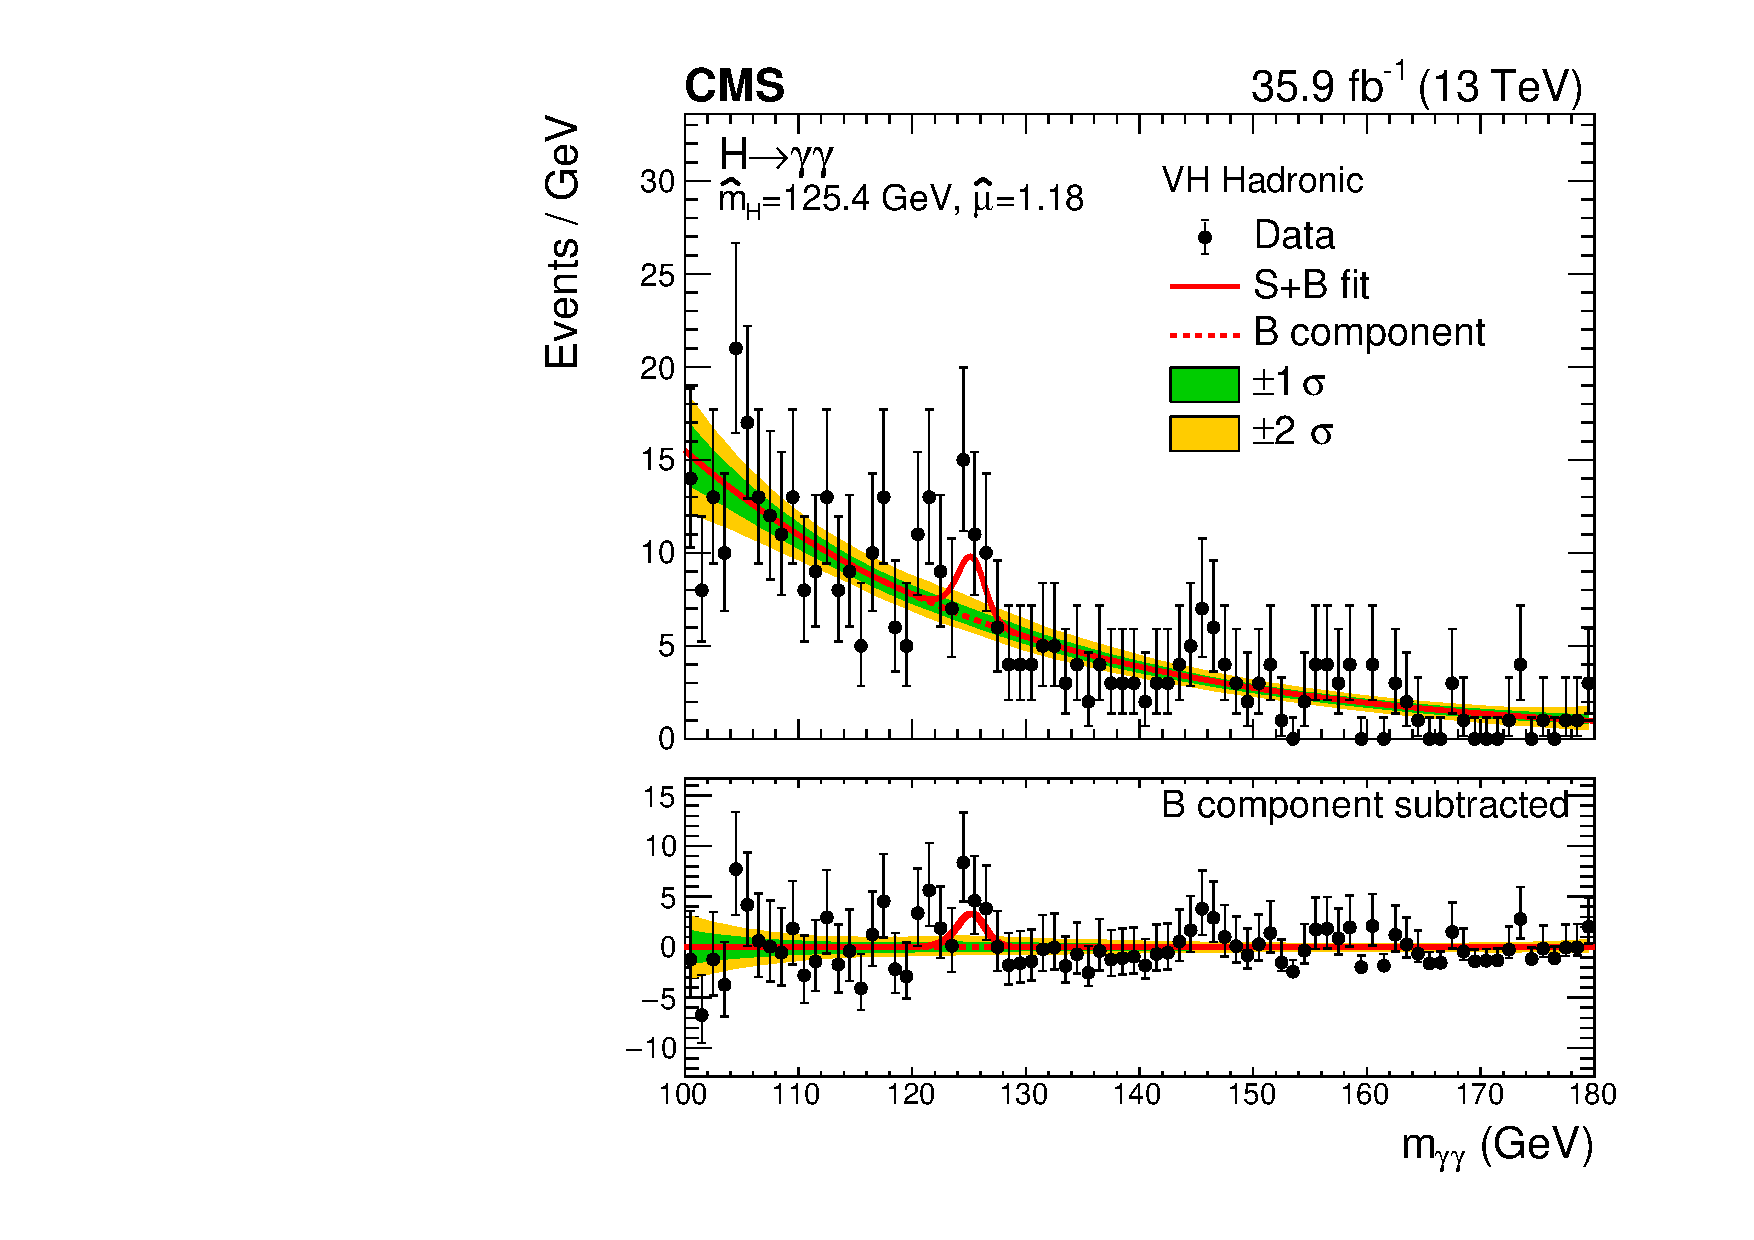
\includegraphics[width=0.47\textwidth]{figures/appendix_mass_plots/CMS-HIG-16-040_Figure_013-e.pdf}
        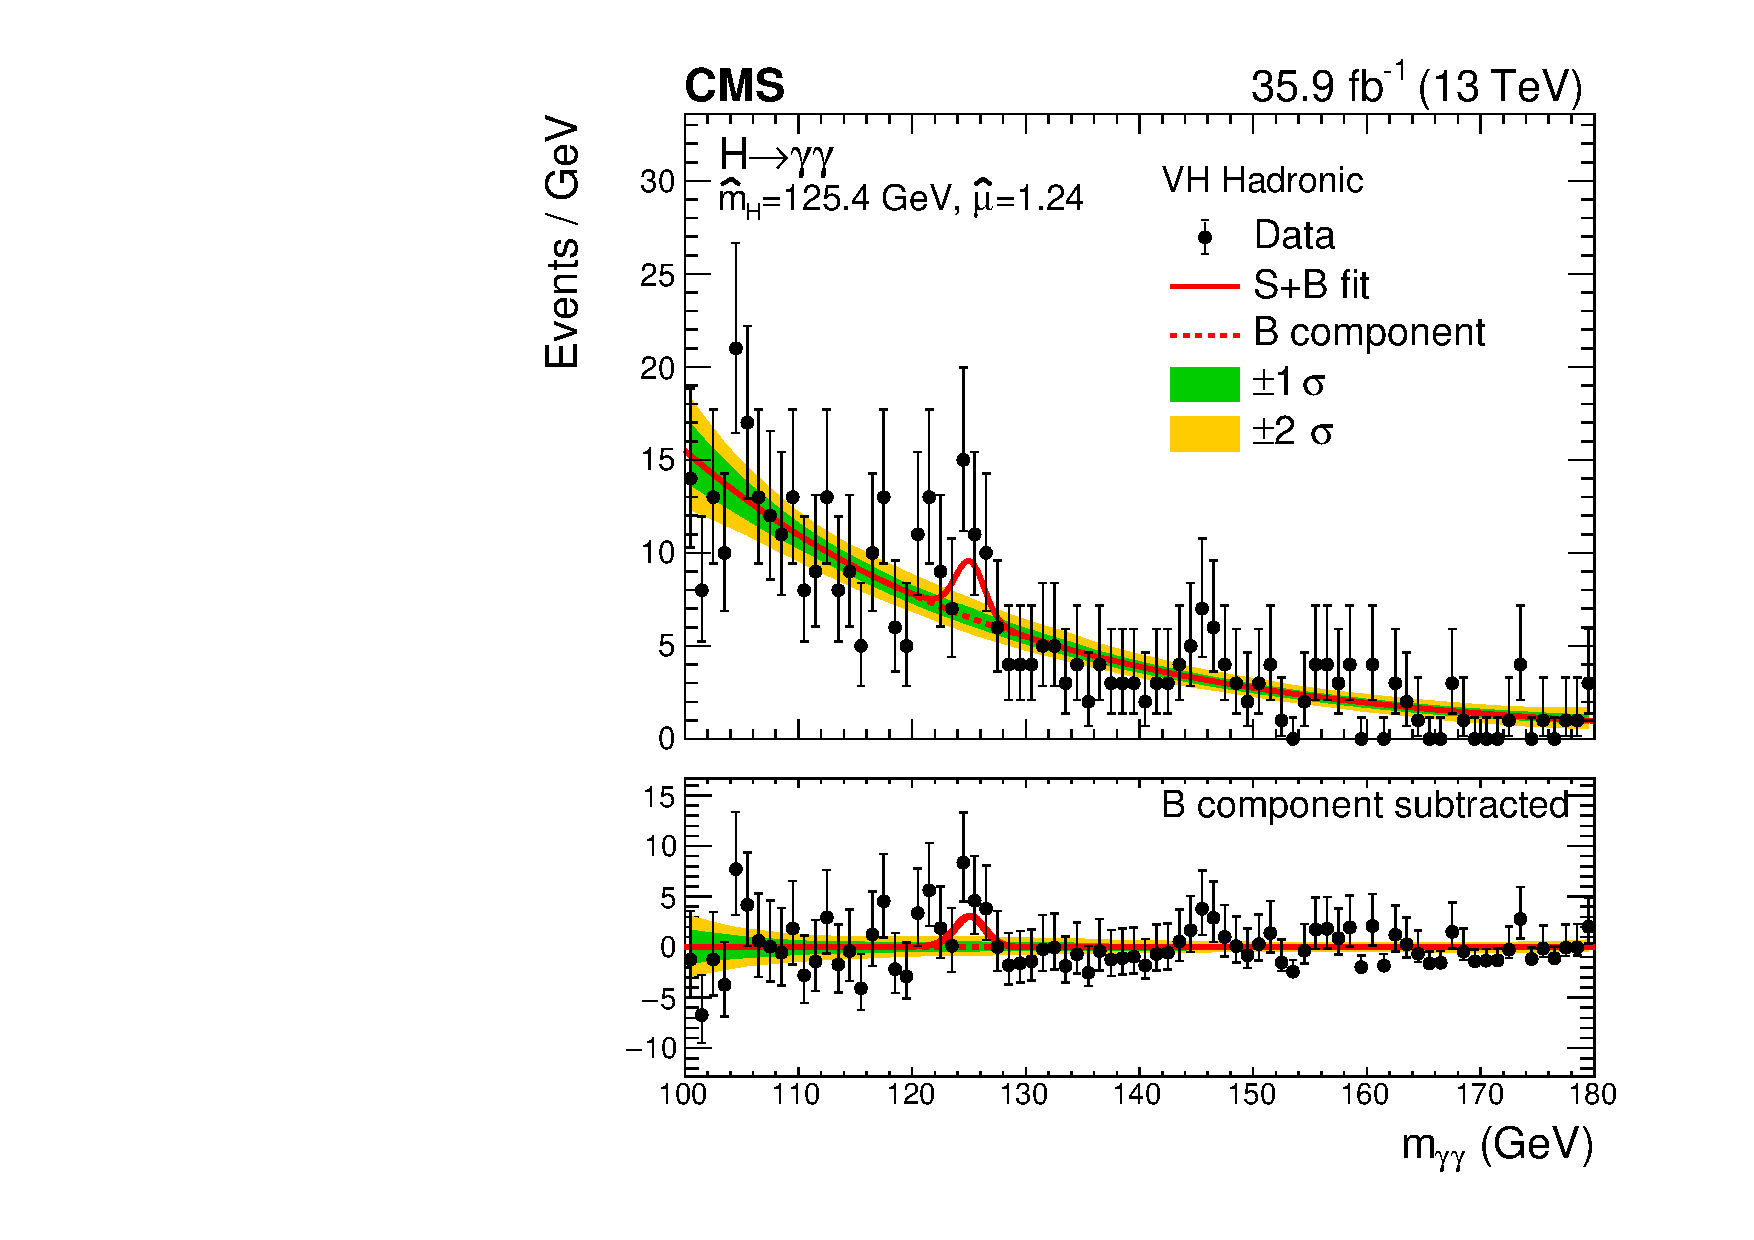
\includegraphics[width=0.47\textwidth]{figures/appendix_mass_plots/SBplots_jackWSnewOldTTHVHHadronicTag_13TeV.pdf}
    \end{center}
    \caption{VH MET and VH hadronic tags. BDT-based VBF analysis is on the left and DCNN-based is on the right.}
        \label{fig:app_mass_plots:vh_met_had}
\end{figure}

\begin{figure}[h!]
    \begin{center}
        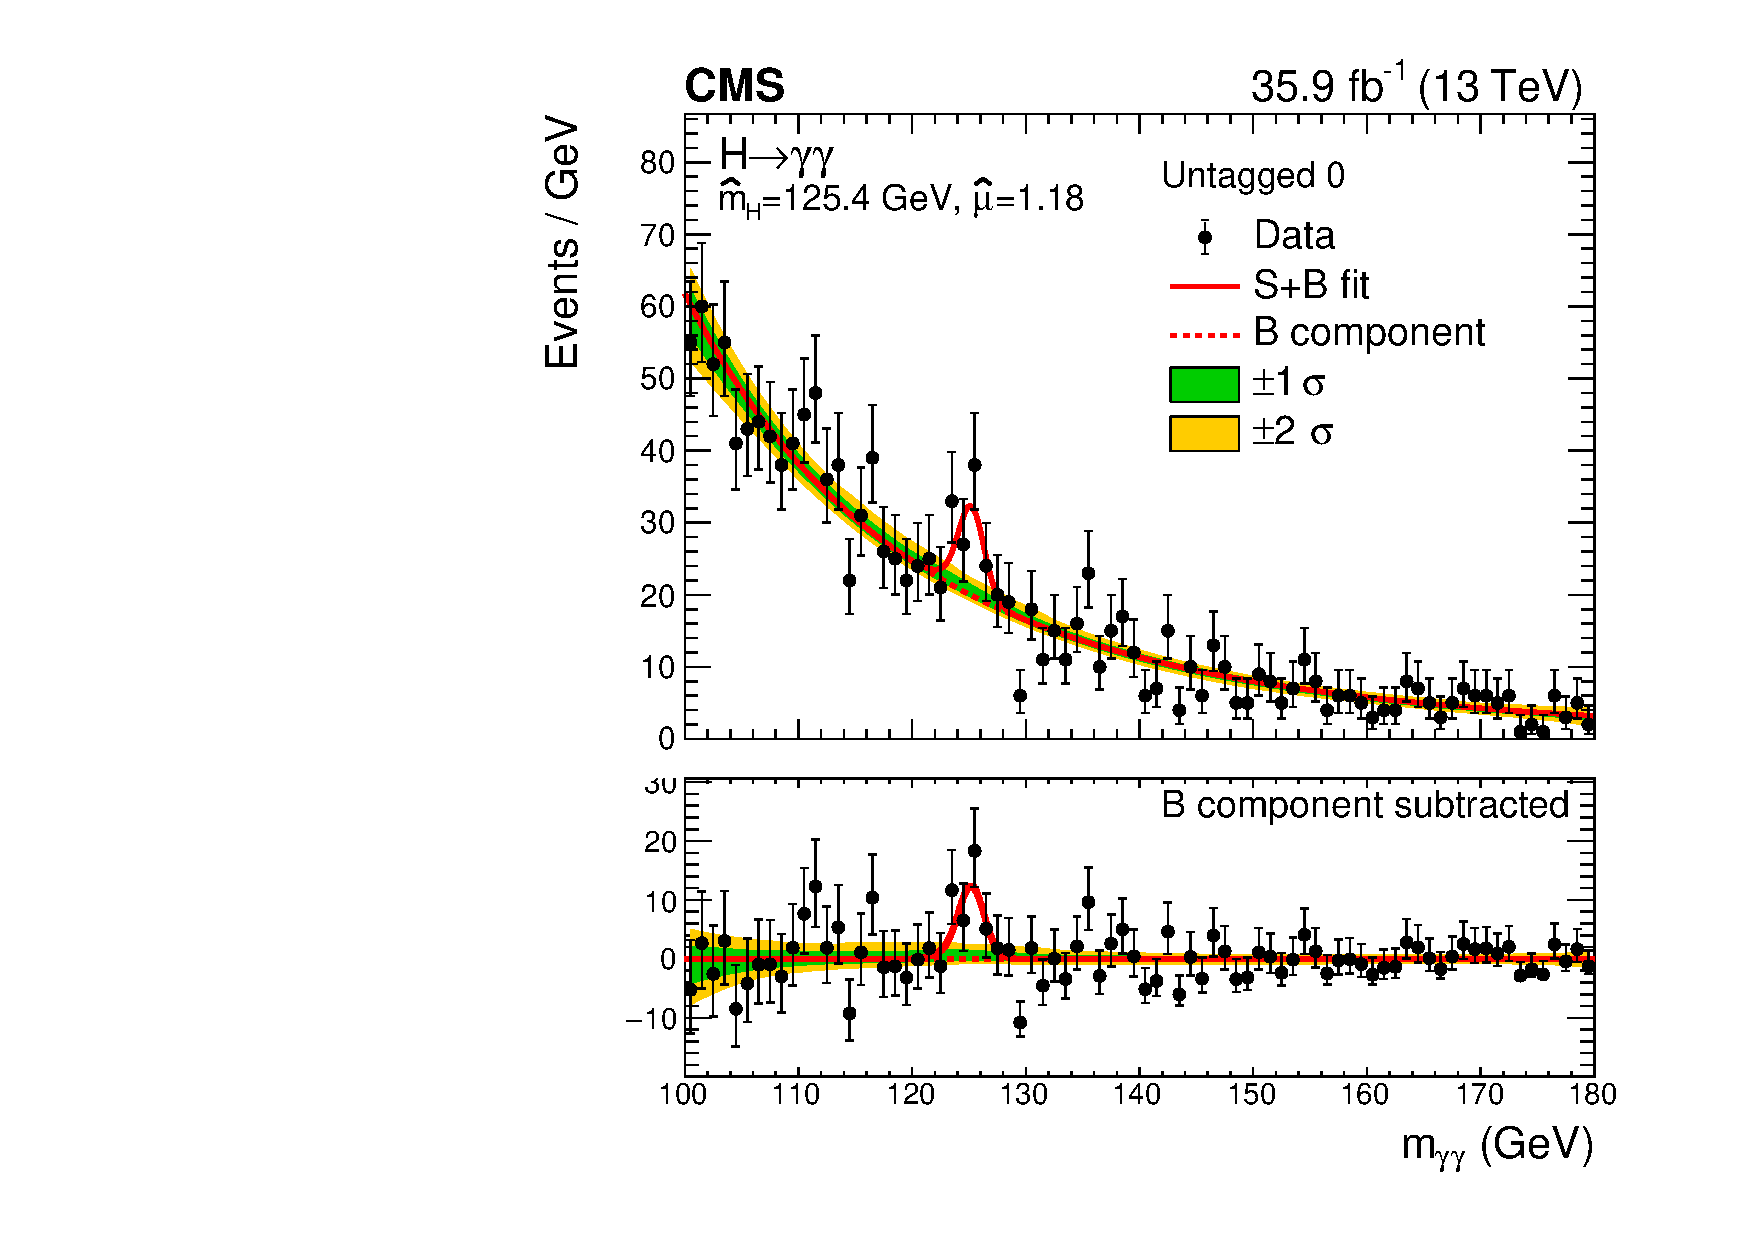
\includegraphics[width=0.47\textwidth]{figures/appendix_mass_plots/CMS-HIG-16-040_Figure_011-a.pdf}
        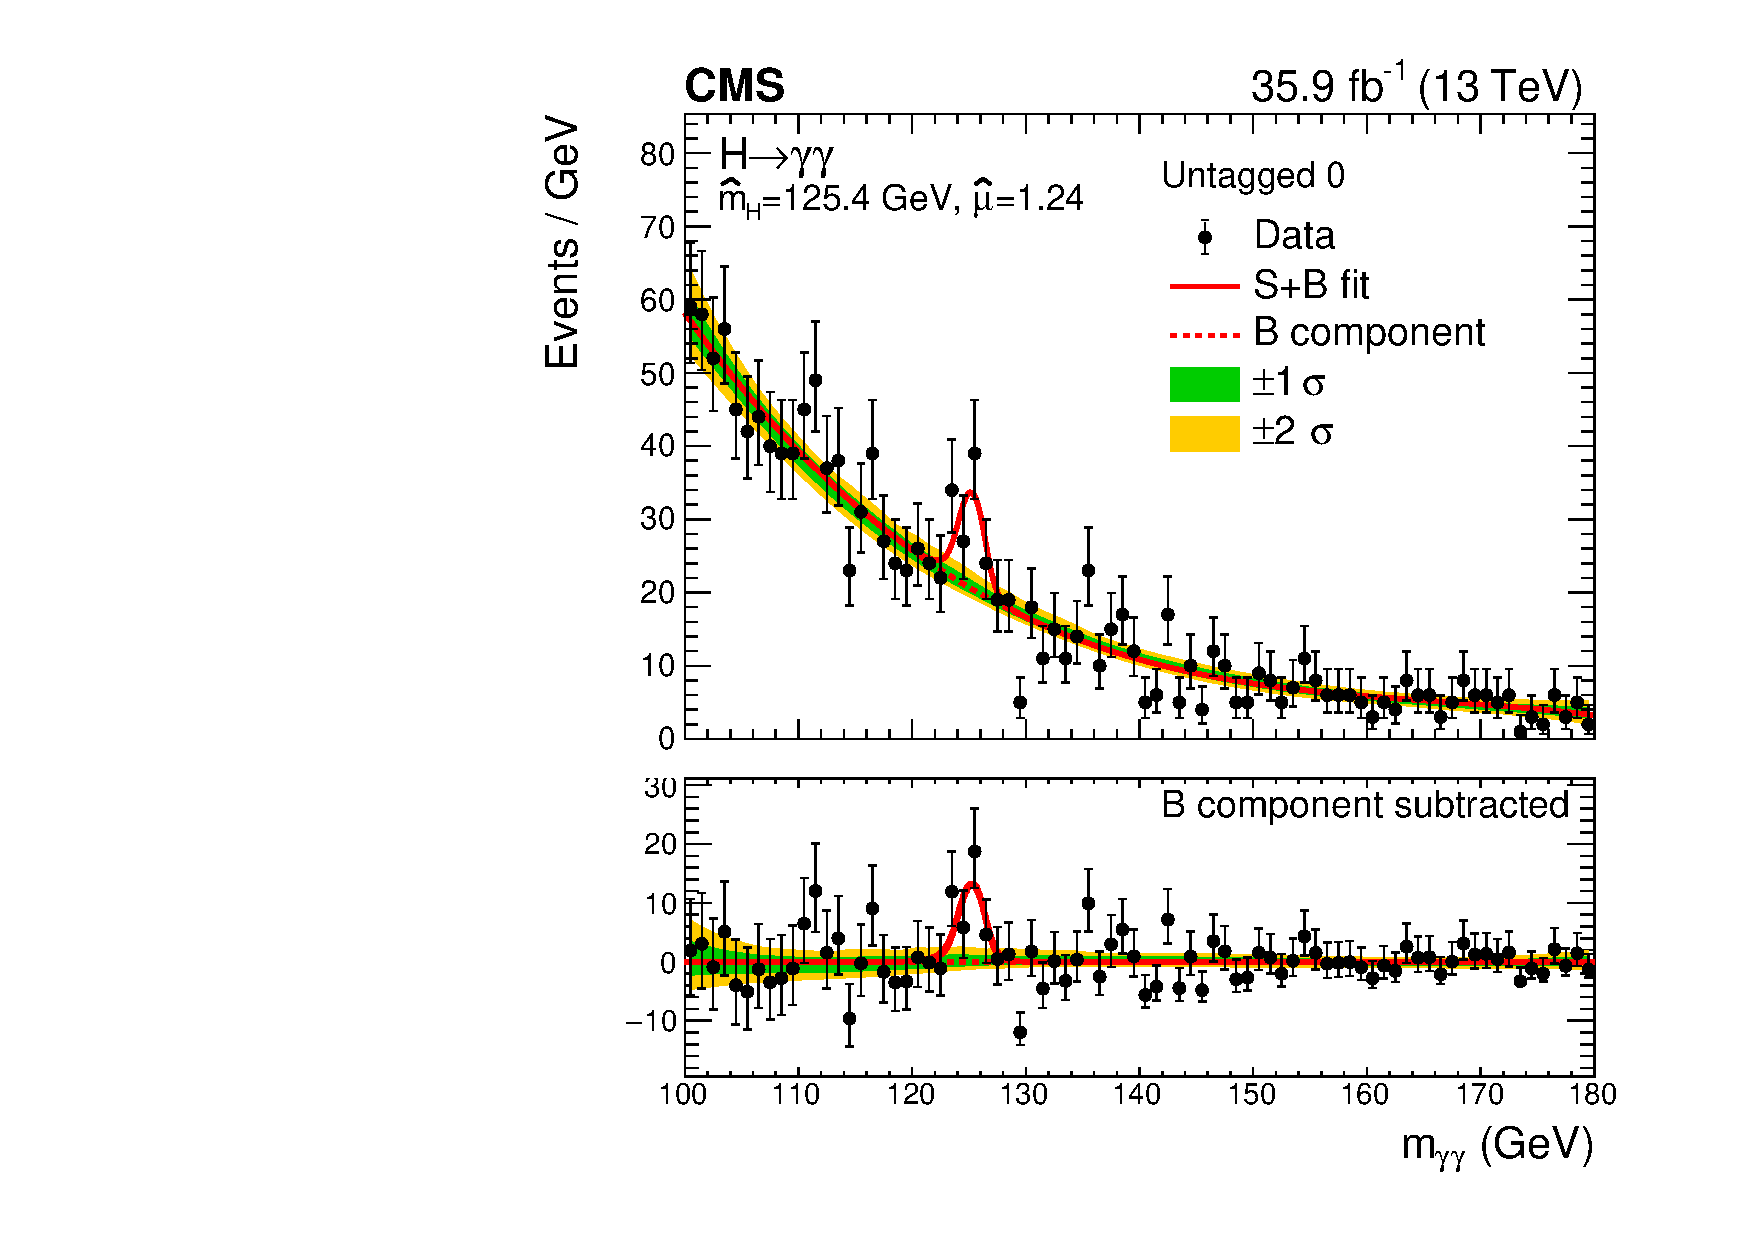
\includegraphics[width=0.47\textwidth]{figures/appendix_mass_plots/SBplots_jackWSnewOldTTHUntaggedTag_0_13TeV.pdf}
    \end{center}
    \begin{center}
        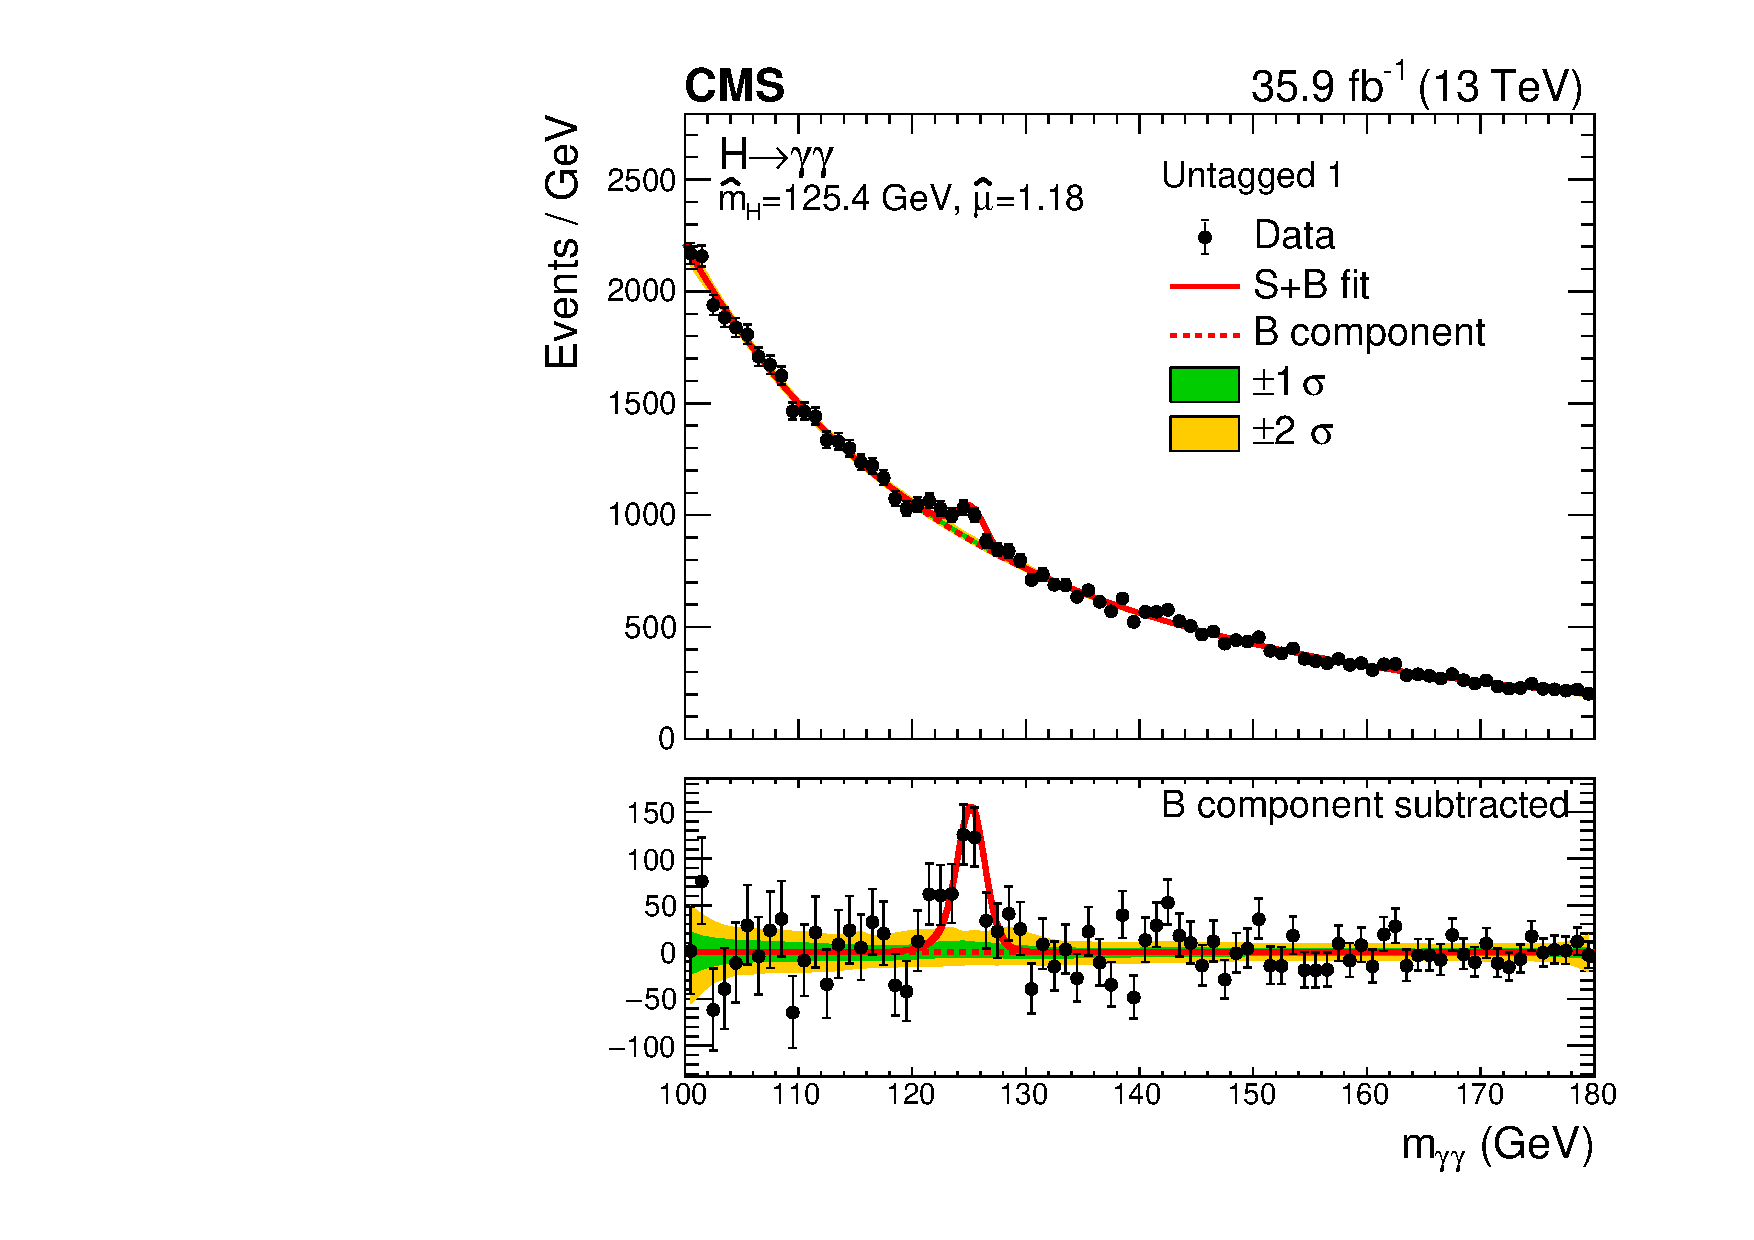
\includegraphics[width=0.47\textwidth]{figures/appendix_mass_plots/CMS-HIG-16-040_Figure_011-b.pdf}
        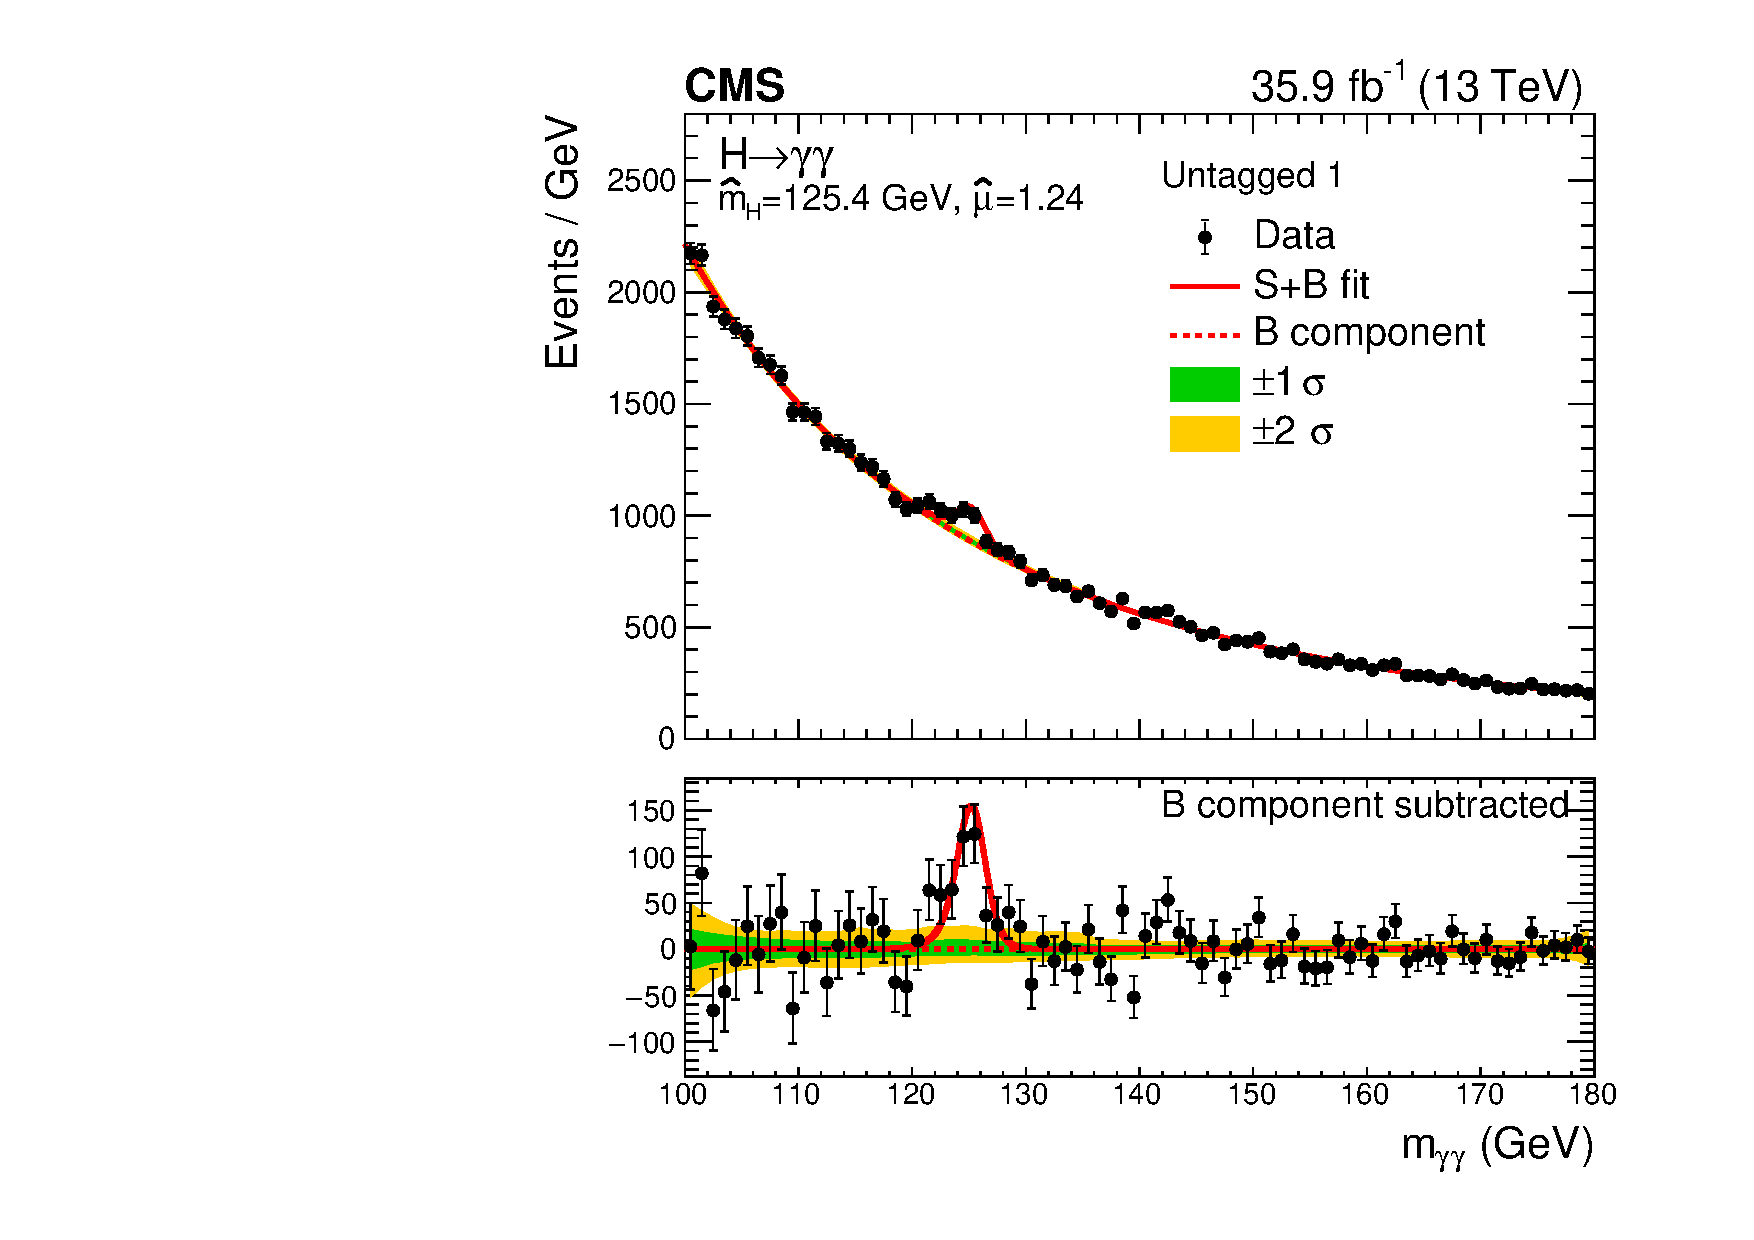
\includegraphics[width=0.47\textwidth]{figures/appendix_mass_plots/SBplots_jackWSnewOldTTHUntaggedTag_1_13TeV.pdf}
    \end{center}
    \caption{Untagged categories 0 and 1. BDT-based VBF analysis is on the left and DCNN-based is on the right.}
        \label{fig:app_mass_plots:unt_0_1}
\end{figure}

\begin{figure}[h!]
    \begin{center}
        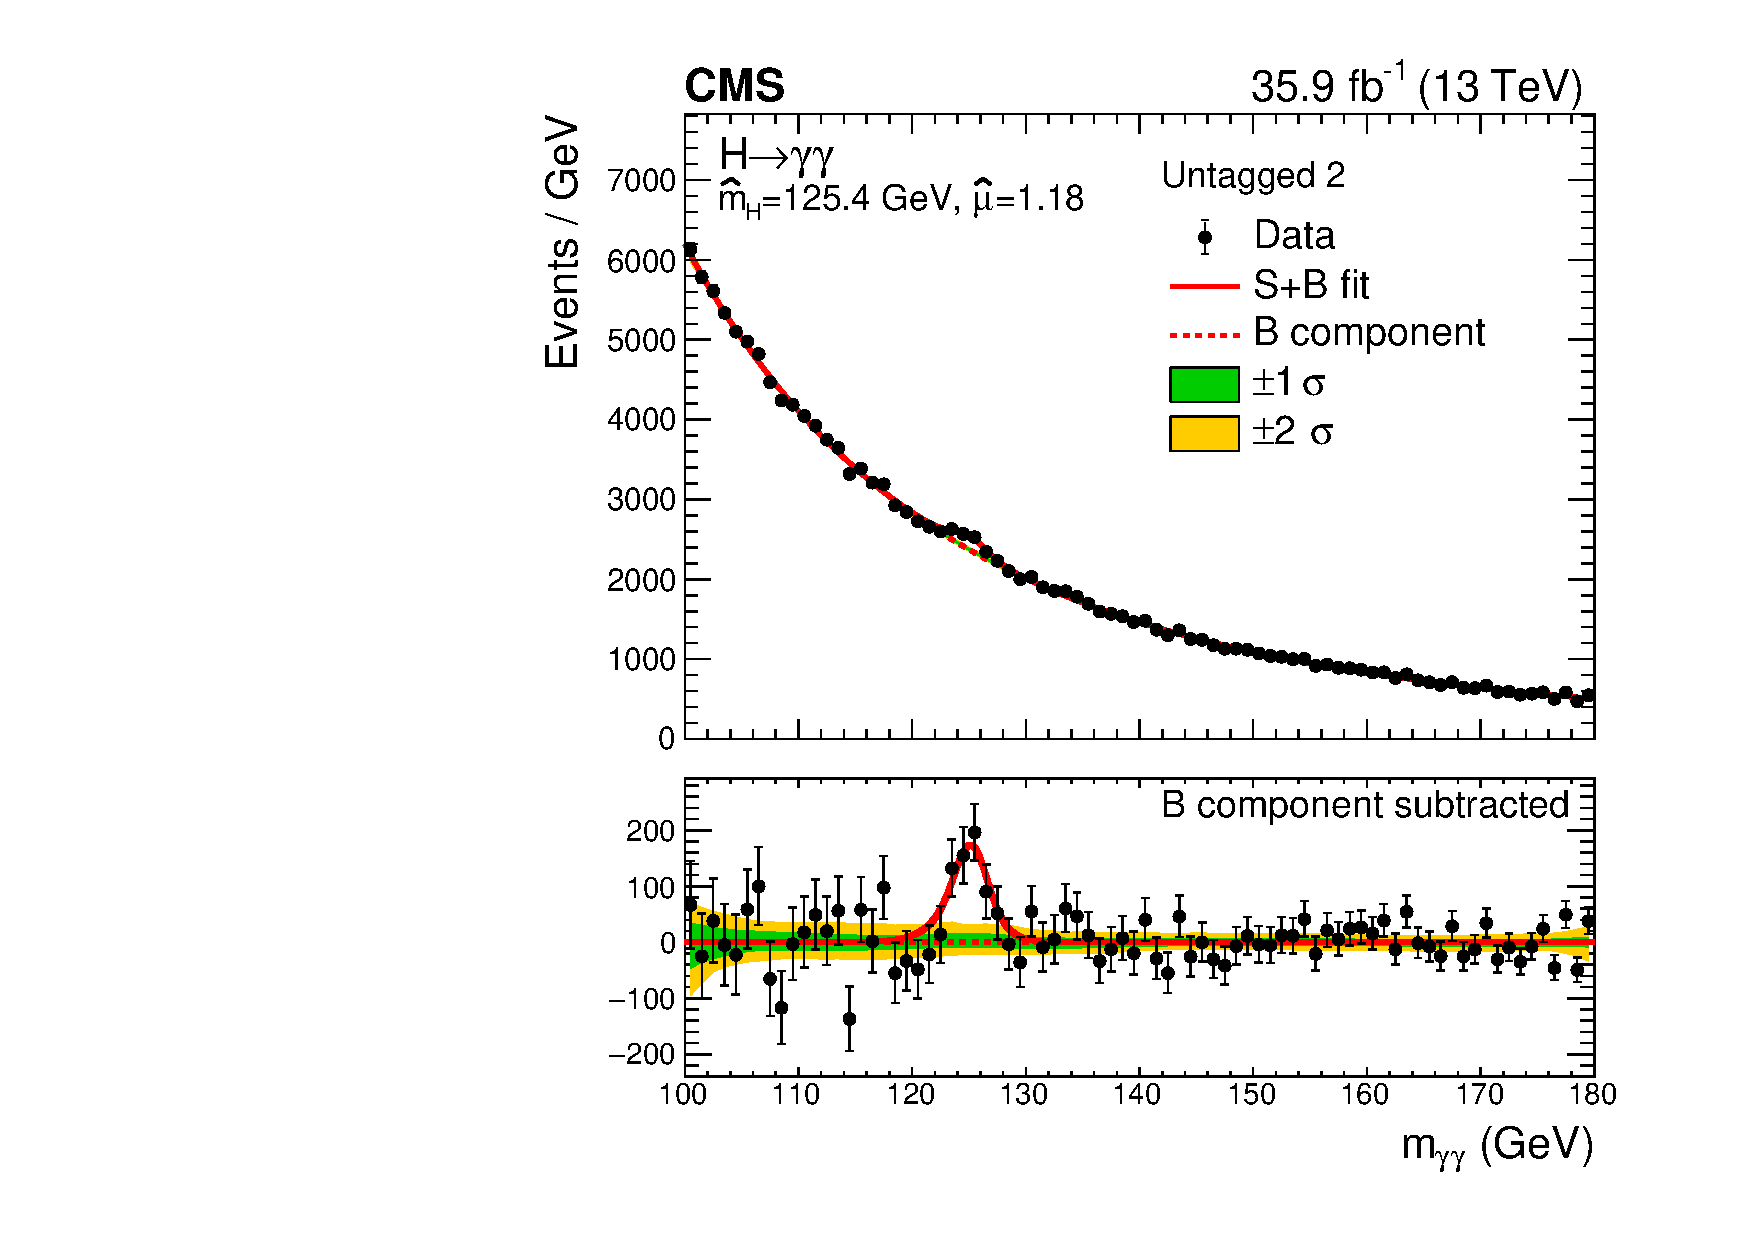
\includegraphics[width=0.47\textwidth]{figures/appendix_mass_plots/CMS-HIG-16-040_Figure_011-c.pdf}
        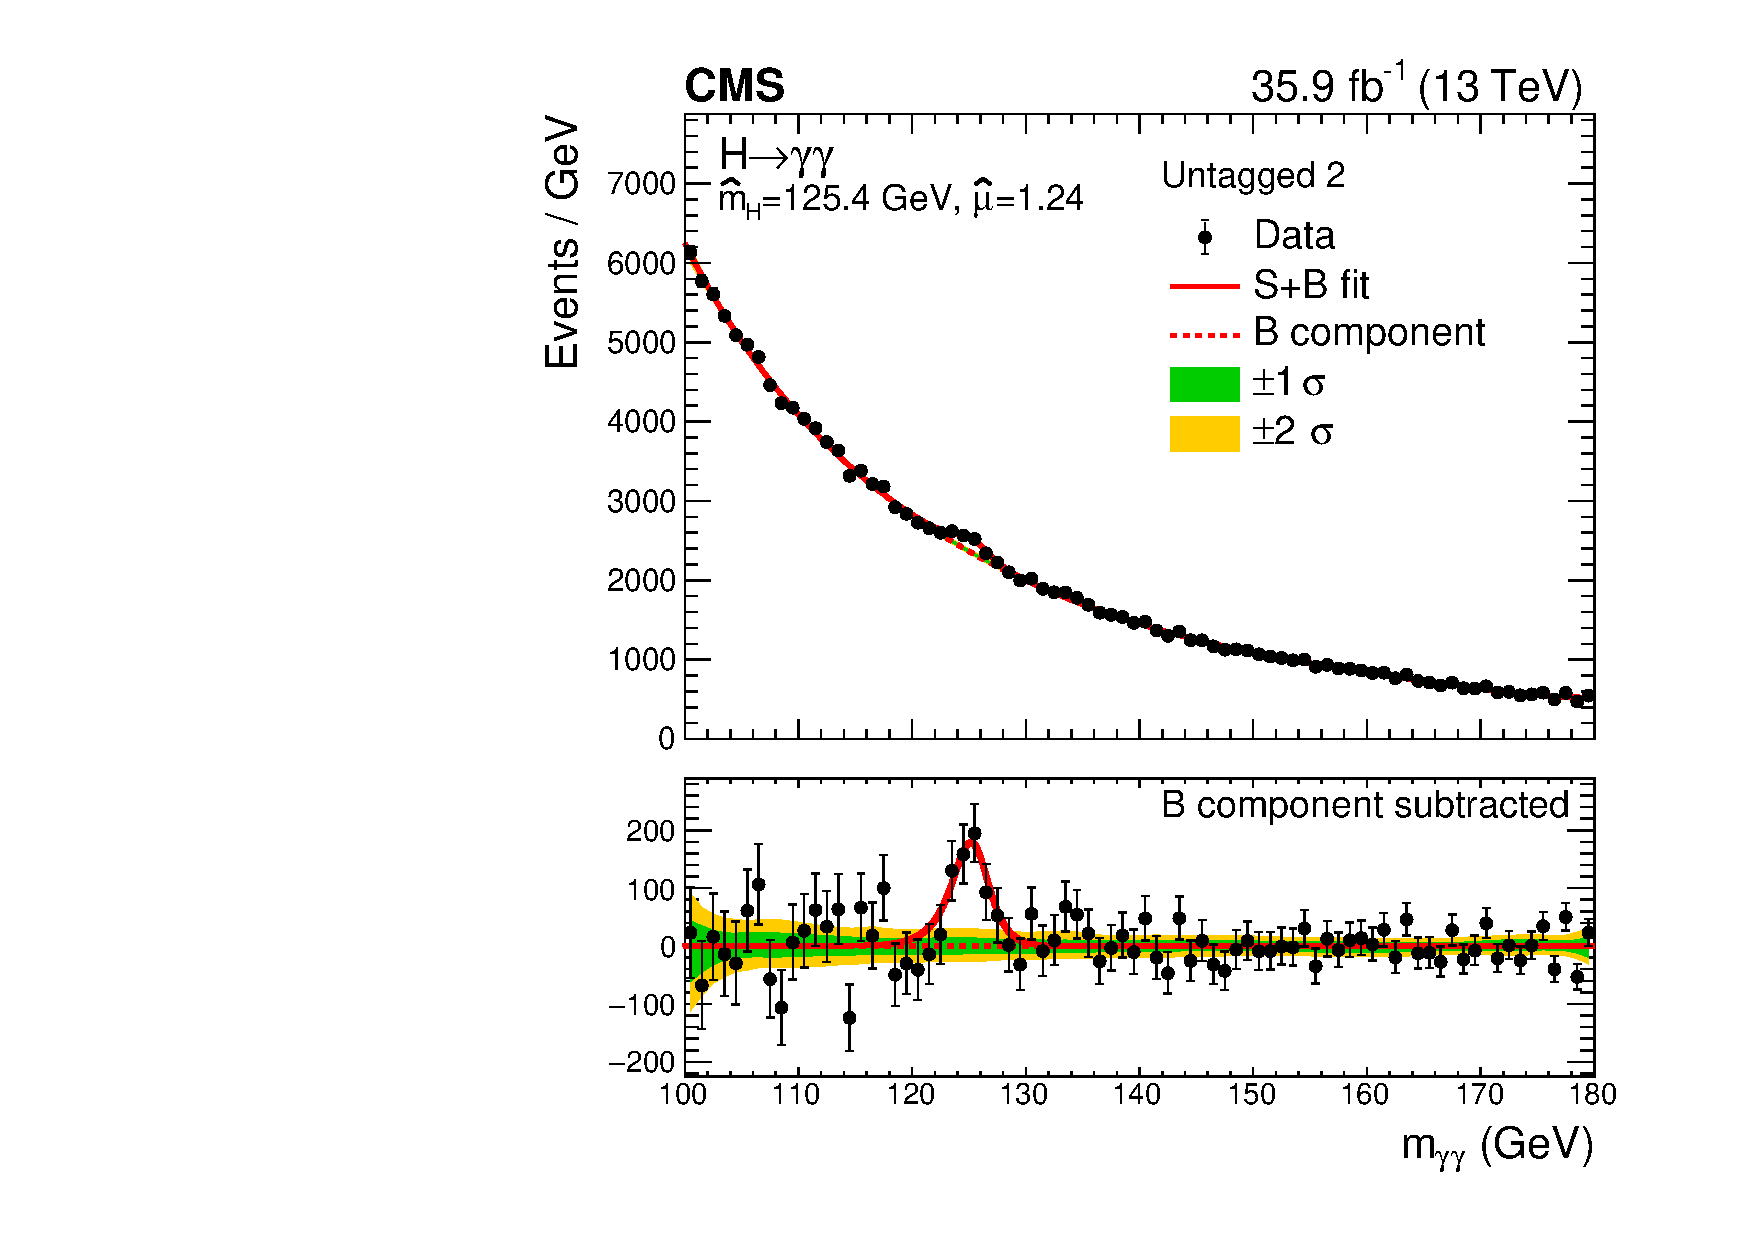
\includegraphics[width=0.47\textwidth]{figures/appendix_mass_plots/SBplots_jackWSnewOldTTHUntaggedTag_2_13TeV.pdf}
    \end{center}
    \begin{center}
        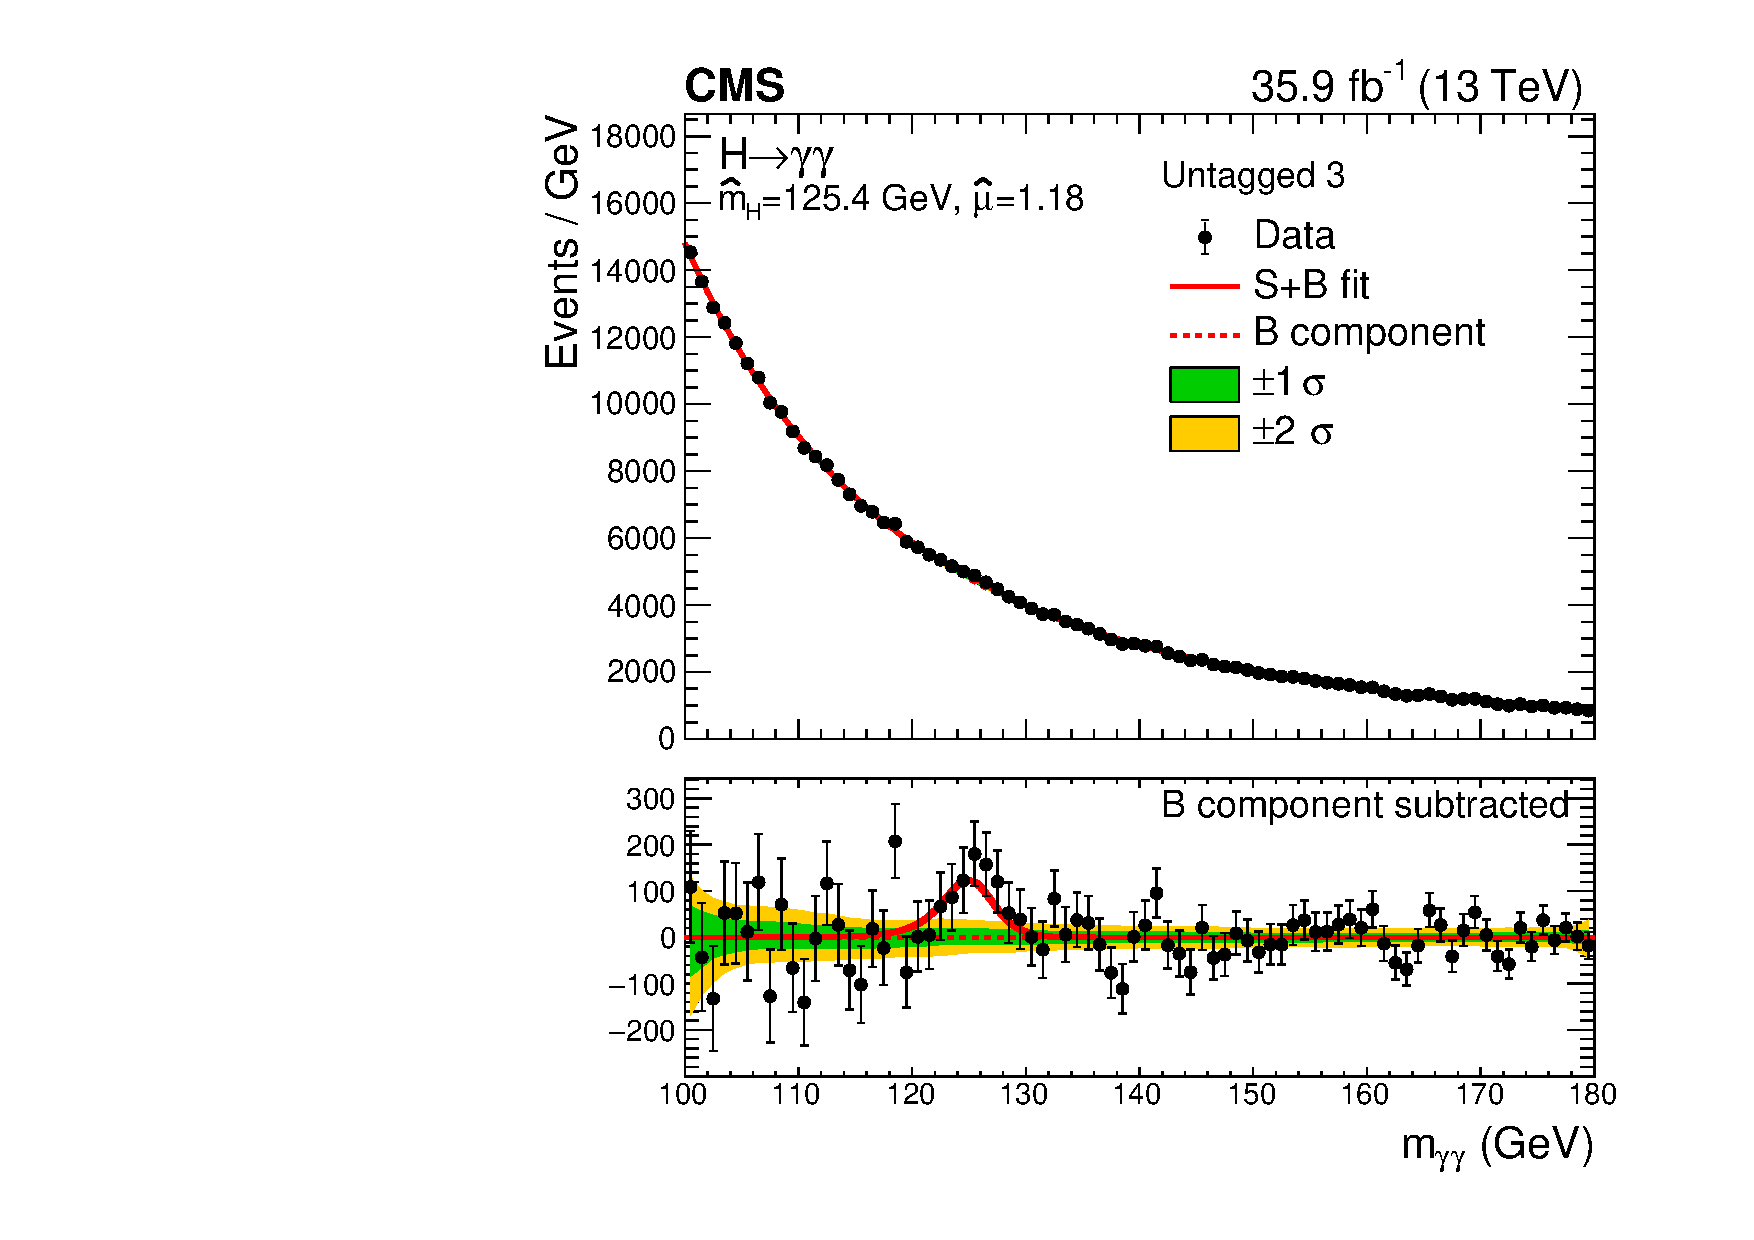
\includegraphics[width=0.47\textwidth]{figures/appendix_mass_plots/CMS-HIG-16-040_Figure_011-d.pdf}
        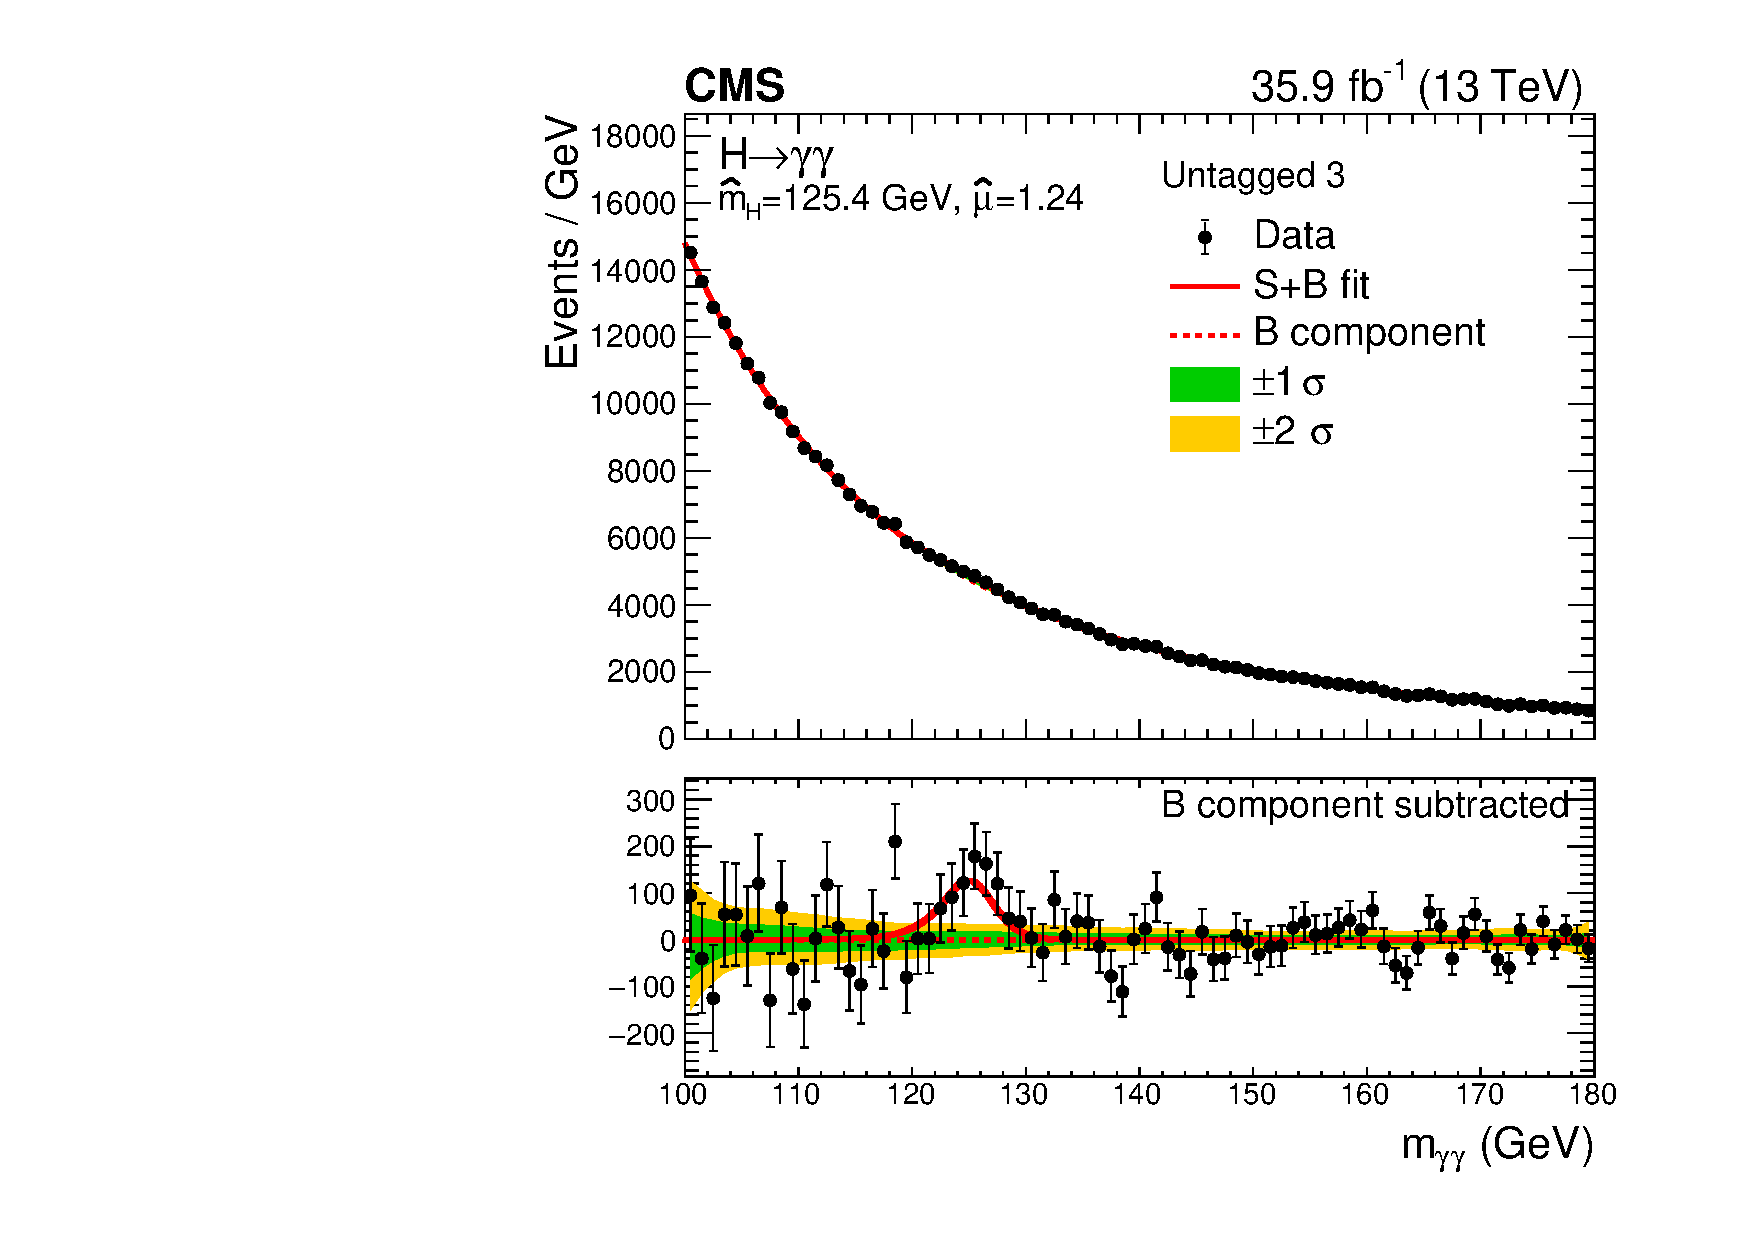
\includegraphics[width=0.47\textwidth]{figures/appendix_mass_plots/SBplots_jackWSnewOldTTHUntaggedTag_3_13TeV.pdf}
    \end{center}
    \caption{Untagged categories 2 and 3. BDT-based VBF analysis is on the left and DCNN-based is on the right.}
        \label{fig:app_mass_plots:unt_2_3}
\end{figure}






